%%%%%%%% ICML 2019 EXAMPLE LATEX SUBMISSION FILE %%%%%%%%%%%%%%%%%

\documentclass{article}

% Recommended, but optional, packages for figures and better typesetting:
\usepackage{microtype}
% \usepackage{graphicx}
\usepackage{subfigure}
\usepackage{booktabs} % for professional tables

% hyperref makes hyperlinks in the resulting PDF.
% If your build breaks (sometimes temporarily if a hyperlink spans a page)
% please comment out the following usepackage line and replace
% \usepackage{icml2019} with \usepackage[nohyperref]{icml2019} above.
\usepackage{hyperref}

% Attempt to make hyperref and algorithmic work together better:
\newcommand{\theHalgorithm}{\arabic{algorithm}}

% \usepackage{icml2019}
\usepackage{icml2019}
\usepackage{wrapfig}
\usepackage{amsfonts}
\usepackage{amsmath}
\usepackage{amssymb}
\usepackage{stmaryrd}
\usepackage{graphicx}
\usepackage{fancyvrb}
\usepackage{amsthm}
\usepackage{mathtools}
\usepackage{bm}
\usepackage{array}
\usepackage{enumitem}
\usepackage{proof}


\theoremstyle{definition} % amsthm only
\newtheorem{definition}{Definition}
\newtheorem{example}{Example}
\newtheorem{proposition}{Proposition}
\newtheorem{algowizm}{Algorithm}
\newtheorem{theorem}{Theorem}
\graphicspath{{figures/}}

\newcommand{\PE}{\textsc{PE}}

\DeclareMathOperator*{\argmin}{arg\,min}
\DeclareMathOperator*{\argmax}{arg\,max}
\DeclareMathOperator{\clip}{clip}
\DeclareMathOperator{\abs}{abs}
\DeclareMathOperator{\dupl}{dupl}
\DeclareMathOperator{\sqr}{sqr}
\DeclareMathOperator{\mean}{mean}
\DeclareMathOperator{\gathernd}{gather}
\DeclareMathOperator{\scatter}{scatter}
\DeclareMathOperator{\reshape}{reshape}
\DeclareMathOperator{\lk}{\ell}


\newcommand{\ciidg}[1]{\textrm{ciidgroup}({#1})}

% \newcommand{\soft}[1]{\tilde{#1}}
% \newcommand{\soft}[1]{\stackrel{\sim}{#1}}
\newcommand{\soft}[1]{\mathrel{\tilde{#1}}}
\newcommand{\dsoft}[1]{\mathrel{\tilde{#1}}}


\usepackage{accents}
% \newcommand{\dsoft}[1]{\stackrel{\approx}{#1}}
% \newcommand{\dsoft}[1]{\accentset{\approx}{#1}}
% \newcommand{\dsoft}[1]{\approx{#1}}

\newcommand{\card}[1]{\left\vert {#1} \right\vert}
\newcommand{\apinv}[1]{\widetilde{#1}^{-1}}
\newcommand{\norm}[1]{\left\|{{#1}}\right\|}
% \newcommand{\pre}[1]{{#1}^{\leftarrow}}
\newcommand{\pre}[2]{{#1}^\leftarrow[#2]}
\newcommand*\wc{{\mkern 2mu\cdot\mkern 2mu}}

\newcommand{\inlinecode}{\texttt}
\newcommand{\alio}{Ali\=o}
\newcommand{\invmap}{\inlinecode{invmap}}
\newcommand*\vmn{{_{m}v_{n}}}

\newcommand*\equ{\overset {\underset {\mathrm {def} }{}}{=}}

% commands to define functions in algorithmic


\DeclareMathOperator{\hire}{offer}

\DeclareMathOperator{\Real}{Real}
\DeclareMathOperator{\Int}{Int}
\DeclareMathOperator{\Bool}{Bool}
\DeclareMathOperator{\cond}{cond}
\DeclareMathOperator{\lift}{lift}
\DeclareMathOperator{\rcd}{rcd}
\DeclareMathOperator{\uw}{uw}
\DeclareMathOperator{\rid}{rid}
\DeclareMathOperator{\iid}{iid}
\DeclareMathOperator{\ciid}{ciid}
\DeclareMathOperator{\fix}{fix}
\DeclareMathOperator{\doo}{do}
% \DeclareMathOperator{\soft}{soft}
\DeclareMathOperator{\rand}{rand}
\DeclareMathOperator{\true}{true}
\DeclareMathOperator{\false}{false}
\DeclareMathOperator{\uid}{newid}
\DeclareMathOperator{\uuid}{uid}
\DeclareMathOperator{\id}{id}
\DeclareMathOperator{\guid}{newid}
\DeclareMathOperator{\pair}{mix}
\DeclareMathOperator{\var}{Var}

\DeclareMathOperator{\bern}{Bern}
\DeclareMathOperator{\unif}{Unif}

\DeclareMathOperator{\stdunif}{unif}
\DeclareMathOperator{\sumunif}{sumunif}
\DeclareMathOperator{\rade}{Rademacher}
\DeclareMathOperator{\normal}{\mathcal{N}}
\DeclareMathOperator{\ee}{\mathbb{E}}
\DeclareMathOperator{\prob}{\mathbb{P}}
\DeclareMathOperator{\rv}{rv}
\DeclareMathOperator{\RV}{RV}
\DeclareMathOperator{\ro}{rand\Omega}

\DeclareMathOperator{\erra}{error}
\DeclareMathOperator{\dq}{:=}
\DeclareMathOperator{\mrg}{merge}
\DeclareMathOperator{\der}{derivation}
\DeclareMathOperator{\ance}{ancestors}

\newcommand{\pushenv}[2]{\Gamma, #1 : #2}
\newcommand{\eto}[2]{#1 \mapsto #2}
\newcommand{\ceto}[3]{#1,  #2 \mapsto #3}
\newcommand{\crv}[3]{(#1, #2, #3)}
\newcommand{\crvv}[2]{\langle#1, #2\rangle}

% Substitute 1 for 2 in 3
\newcommand{\sub}[3]{#3[#1 / #2]}


\newcommand{\RVT}[1]{\RV #1}

% \DeclareMathOperator{\bern}{bern}

% \theoremstyle{definition} % amsthm only
% \newtheorem{definition}{Definition}
% \newtheorem{example}{Example}
% \newtheorem{proposition}{Proposition}
% \newtheorem{theorem}{Theorem}
% \newtheorem{algowizm}{Algorithm}


\newcommand{\indep}{\perp \!\!\!\perp}
\newcommand{\deq}{\stackrel {d}{=}}
\newcommand{\g}{\,\vert\,}
\newcommand{\cM}{{\mathcal{M}}}
\newcommand{\omegalang}{\textsc{Omega}}
\newcommand{\ite}[3]{\text{ if } #1 \text{ then } #2 \text{ else } #3}
\newcommand{\lifted}[1] {\tilde{#1}}
\newcommand{\amean}[1] {\ee[#1]}
\newcommand{\lmean}[1] {\lifted{\ee}{(#1)}}
% \newcommand{\conds}[2] {#1_{\mid #2}}
\newcommand{\conds}[2] {#1  \mid #2}
\newcommand{\cnd}[2] {#1  \mid #2}
% \newcommand{\rcdxy}[2] {#1\und  erset{\rcd}{\vert}#2}
% \newcommand{\rcdxy}[2] {#1 \tilde{\mid} #2}
\newcommand{\rcdxy}[2] {#1 \parallel #2}
\newcommand{\ridxy}[2] {#1 \parallel \doo(#2)}

\newcommand{\ciidset}[2]{\left[#1\right]_{\indep \mid #2}}


\newcommand{\rom}{\rand_\omega}

% TODO
\usepackage[colorinlistoftodos,prependcaption,textsize=tiny]{todonotes}
\usepackage{xargs} % Use more than one optional parameter in a new commands

% \usepackage[bordercolor=white,backgroundcolor=gray!30,linecolor=black,colorinlistoftodos]{todonotes}
\newcommand{\rework}[1]{\todo[color=yellow,inline]{Rework: #1}}
% \newcommand{\wtp}[1]{\todo[color=cyan,inline]{Write about: #1}}

\newcommandx{\unsure}[2][1=]{\todo[linecolor=red,backgroundcolor=red!25,bordercolor=red,#1]{#2}}
\newcommandx{\change}[2][1=]{\todo[linecolor=blue,backgroundcolor=blue!25,bordercolor=blue,#1]{#2}}
\newcommandx{\info}[2][1=]{\todo[linecolor=OliveGreen,backgroundcolor=OliveGreen!25,bordercolor=OliveGreen,#1]{#2}}
\newcommandx{\improvement}[2][1=]{\todo[linecolor=Plum,backgroundcolor=Plum!25,bordercolor=Plum,#1]{#2}}
\newcommandx{\wtp}[2][1=]{\todo[linecolor=orange,backgroundcolor=orange!25,bordercolor=orange,#1]{#2}}
\newcommandx{\thiswillnotshow}[2][1=]{\todo[disable,#1]{#2}}


\newenvironment{code}
{\begin{figure}[H]
\centering
\begin{BVerbatim}}
{\end{BVerbatim}
\end{figure}}

% \newenvironment{code}{start}{stop}

\newcommand{\bigcomment}[2]{
  \begin{center}
  \fbox{\begin{minipage}{\linewidth}{\bf #1:} {\rm #2}\end{minipage}}
  \end{center}
}

\newcommand{\XZ}[1]{\bigcomment{XZ}{#1}}


\makeatletter
\newenvironment{exprogram}[1][htb]{%
    \renewcommand{\ALG@name}{Example Program}% Update algorithm name
   \begin{algorithm}[#1]%
  }{\end{algorithm}}
\makeatother

\makeatletter
\newcommand{\ALOOP}[1]{\ALC@it\algorithmicloop\ #1%
  \begin{ALC@loop}}
\newcommand{\ENDALOOP}{\end{ALC@loop}\ALC@it\algorithmicendloop}
\makeatother

\renewcommand{\algorithmicloop}{\textbf{subroutine}}

% If accepted, instead use the following line for the camera-ready submission:
\usepackage{icml2019}

% The \icmltitle you define below is probably too long as a header.
% Therefore, a short form for the running title is supplied here:
\icmltitlerunning{Soft Constraints for Inference with Declarative Knowledge}
% \usepackage[dvipdfm]{graphicx}
% \usepackage{bmpsize}
\begin{document}

\twocolumn[
\icmltitle{Soft Constraints for Inference with Declarative Knowledge}

% It is OKAY to include author information, even for blind
% submissions: the style file will automatically remove it for you
% unless you've provided the [accepted] option to the icml2019
% package.

% List of affiliations: The first argument should be a (short)
% identifier you will use later to specify author affiliations
% Academic affiliations should list Department, University, City, Region, Country
% Industry affiliations should list Company, City, Region, Country

% You can specify symbols, otherwise they are numbered in order.
% Ideally, you should not use this facility. Affiliations will be numbered
% in order of appearance and this is the preferred way.
\icmlsetsymbol{equal}{*}

\begin{icmlauthorlist}
\icmlauthor{Zenna Tavares}{mit}
\icmlauthor{Javier Burroni}{amhert}
\icmlauthor{Edgar Minaysan}{princeton}
\icmlauthor{Armando Solar Lezama}{mit}
\icmlauthor{Rajesh Ranganath}{nyu}
\end{icmlauthorlist}

\icmlaffiliation{mit}{MIT, USA}
\icmlaffiliation{nyu}{NYU, USA}
\icmlaffiliation{amhert}{UMass Amherst, USA}
\icmlaffiliation{princeton}{Princeton University, USA}

\icmlcorrespondingauthor{Zenna Tavares}{zenna@mit.edu}
% \icmlcorrespondingauthor{Eee Pppp}{ep@eden.co.uk}

% You may provide any keywords that you
% find helpful for describing your paper; these are used to populate
% the "keywords" metadata in the PDF but will not be shown in the document
\icmlkeywords{Probabilistic Inference, Markov Chain Monte Carlo, Replica Exchange, Probabilistic Programming}

\vskip 0.3in
]

% this must go after the closing bracket ] following \twocolumn[ ...

% This command actually creates the footnote in the first column
% listing the affiliations and the copyright notice.
% The command takes one argument, which is text to display at the start of the footnote.
% The \icmlEqualContribution command is standard text for equal contribution.
% Remove it (just {}) if you do not need this facility.

%\printAffiliationsAndNotice{}  % leave blank if no need to mention equal contribution
\printAffiliationsAndNotice{\icmlEqualContribution} % otherwise use the standard text.

\section{TODO}
\begin{itemize}
\item (writing) put title back to predicate exchange
\item (writing) abstract needs complete revision (and should be shorter)
\item Possibly remove measure theory, write all in terms of ℓ?
\item proof of propositon 1
\item (relatedwork) add discussion of PSL (in rebuttal)
\item (relatedwork) add discussion of Replica-exchange MCMC (in rebuttal)
\item fix invg depth diagram
\item fix font-size on gaussian plot (figure 7); it's unreadable 
\item (experiments) add complete experimental setup (e.g. num samples, hyperparameter values)
\item (experiments) add MCMC diagnostics, convergence tests, etc
\item (experiments) Another experiment?
\item (figures) more analysis of dynamics of replica exchange
\item theorem / proof of correctness of replica exchange algorithm
\item expand on naming/ids
\item replace x = normal(x, 0, 1) with x = normal(xid, 0, 1)
\item expand on loops,control-flow with examples
\end{itemize}

\newpage

\begin{abstract}
We develop a likelihood free inference procedure for conditioning a probabilistic model on a predicate.
A predicate is a Boolean valued function which expresses a yes/no question about a domain.
When a model is conditioned on a predicate, the model is revised such that the predicate becomes a true proposition.
An observation is a special kind of predicate, that is true if and only if a variable is equal to a value.
Predicates can express propositions other than the observation of data.
For instance, they can assert constraints on latent variables, rather than observables.
They can express observations that are more coarse than variables in the model.
Furthermore, predicates can be combined together in complex logical combinations.
Unfortunately, conditioning a model on a predicates remains severely limited due to the fact that the corresponding likelihood is often intractable to compute, if it is available at all.
Our contribution, which we call predicate exchange, 
constructs a softened predicate which takes value in the unit interval [0, 1] as opposed to simply true or false. Intuitively, 1 corresponds to true, and a high value (such as 0.999) corresponds to "nearly true" as determined by a distance metric.
We define Boolean algebra for soft predicates,  such that they can be negated, conjoined and disjoined arbitrarily.
A softened predicate can serve as a tractable proxy to a likelihood function for approximate posterior inference.
However, we target exact inference by tempering the relaxation by a temperature parameter, and use replica exchange Markov Chain Mont Carlo, which exchanges states between a sequence of models conditioned on predicates at varying temperatures.
In doing so, we are able to draw exact samples from the original, unrelaxed model.
We present a lightweight, a language independent implementation of predicate exchange that modulates the execution of a simulation based model.
Finally, we demonstrate our approach on a number of standard benchmarks and present case studies in inverse graphics, and physiological forecasting.
\end{abstract}

\section{Introduction}

% WTP: What are simulation based models, what is bayesian inference in them.  Why is it necessary. 
% Mechanistic knowledge is well modeled through simulation, whereby values, states, and transitions in the execution of a program correspond to aspects of the process being modeled. 
% Even when equational laws that govern a system are known, simulation models are still useful as an algorithm that computes a solution.

Particularly in the sciences, many phenomena are readily modeled through simulation.
A simulation models a domain as an algorithm which solves the equations which govern it. Values, states, and transitions in the execution of the algorithm correspond to entities in the domain.
Typically, this execution flows causally in the sense that if $a$ causes $b$ in the domain, $b$ is computed from $a$ in simulation.
Inference problems, on the other hand, demand the inverse.
Often we have observed the result of the simulation, and want to infer likely causes.


% % WTP: 
% Many phenomena, particularly in the sciences, are understood mechanistically and hence well modeled through simulation.
% A simulation model is a program, whereby values constructed in its execution correspond to components of the process being modeled. 
% Simulation models generally have forward causal direction; they are executed to produce output from a given input.
% Probability theory 
% % Simulation models express generative processes that construct observable data, and are unique in their ability to capture complex phenomena across a variety of domains, particularly in the sciences.
% Unfortunately, the very flexibility that allows simulation models renders them resistant to many kinds of analysis.
% In particular, the vast majority of algorithms which perform Bayesian inference in probabilistic models -- that is, sample likely values of latent variables given  observed data -- rely on computing the likelihood function, which is not explicitly represented in a simulation model, and more often than not is intractable to compute.

% WTP: What are likelihood functions, why are they use useful, and why are they intractable
The Bayesian approach quantifies all uncertainty with probabilities and as a result uniquely specifies the posterior distribution over latent variables.
% Bayesian inference is a principled framework for inferring probable causes of observed values, but relies on terms which are often intractable.
Most algorithms which draw samples from posterior distributions rely on
% Bayes theorem dictates that the posterior distribution over latent variables given observations is is proportional to the product of the likelihood function and prior.
the likelihood function, which quantifies the extent to which values of latent variables are consistent with observations.
Whereas many probabilistic models are specified explicitly by their likelihood functions, likelihoods are implicit to simulation models and often intractable, i.e., defined by an integral or summation that lacks a closed form solution or is computationally intractable.
This can occur, for example, when non-latent variables are unobserved, since they must be margainalized out.
Alternatively, conditioning deterministic transformations of densities are produces integrals change of variables.
Simulation based models can apply arbitrary, non-injective transformations to their input, and hence induce intractable likelihoods for any or all of these reasons.

A less explored cause of intractability is conditioning on propositions that are not observations in the conventional sense.
% Several likelihood-free inference methods exist.
% but they are largely inapplicable to models which lack a tractable likelihood function because their conditions are non-observational.
% WTP: Underappreciate Reason for Problem: Conditioning on observations
% Observing data is a special case of conditioning. 
To observe data $x$ as the output of a simulation model $X$ is to condition the model on a proposition of the form $X = x$.
There are several propositions that do not conform to this structure, which we would nevertheless like to condition our models on.
% A less explored cause of intractability occurs when we condition on propositions that are not observations of data.
For example, if $X$ and $Y$ are normally distributed random variables, then conditioning on $X = Y$ does not permit a density function, let alone a tractable one.
Conditioning on inequalities such $X > 4$, transformations such $X^2  = 0$, and logical formulas such as  $X = 3 \lor X = 5$ falls outside the domain of virtually all conditional sampling algorithms.
% As a consequence, conditioning in practice is significantly more limited than its theoretical counterpart.

% The value of probabilistic programming systems hinges on how easily a practitioner can encode domain knowledge into a model. Existing probabilistic programming systems support two main mechanisms for encoding knowledge: implicitly in the generative model, and explicitly by conditioning on observations. There are many contexts, however, for which neither of these two mechanisms are sufficient to encode the knowledge that practitioners have about a process.

% WTP: Implications of the Problem

Conditioning is a mechanism to express declarative knowledge.
It allows us to assert facts we know to be true without specifying the means by which they are true.
% Limiting the propositions one can condition on to those with tractable likelihoods severely restricts the kinds of knowledge that we can express.
For example, consider the problem of modeling the evolution of glucose levels over time~\citep{levine2017offline}.
A scientist could define a generative model that captures prior knowledge of how glucose levels evolve over time -- for example, the model may use latent variables to identify when a person eats and the glycemic loads a person consumes, and encode physiological knowledge of how those meals will affect glucose levels.
The scientist could also condition the model on observations of glucose measurements of a given patient and use existing inference algorithms to sample from the posterior distributions over latent variables.
However, there are various pieces of declarative knowledge the scientist may possess which are difficult or impossible to encode in this form.
For instance, she may know that ``human glucose curves are similar across patients'',   is surprisingly challenging even in the most expressive probabilistic programming systems. 
Rather than observations, these propositions are facts which condition the prior.These propositions are not observations; 

% WTP: Non-obvious benefits of solving the problem:  Prior conditioning.
Declarative knowledge has the potential to serve as the bridge between classical parametric models, and recent trend towards nonparameric or highly parameterized families such as deep neural networks.
For example, inverse graphics attempts to infer the three dimensional scene (geometry, lights, camera, etc) which caused an observed image.
A Bayesian formulation of the problem requires a prior distributions over scenes.
Simple parametric stand little chance of capturing the complexity of real world scenes, prompting.




% WTP: Contribution: inference algorithm that supports conditioning on a wider class of propositions
In this paper we present an algorithm that draws samples from generative models that have been conditioned on predicates belonging to a more general class than observation of data.
Predicates, when used as black boxes, provide only sparse information -- the constraint is satisfied or it is not -- and the subset of satisfying constraints is typically vanishingly small.
Our objective is to support conditioning on predicates on spaces for which a natural metric can be defined.
A metric provides more information a measure of the degree of satisfaction, and allows us.

% WTP: Paper summary
In summary we address the problem of conditioning on declarative knowledge.
In more detail:
\begin{itemize}
\item We formalize simulation models in measure-theoretic probability as random variables defined on a shared probability space (section X), and define conditioning as a concentration of measure.
\item We describe our approach to inference, which softens the hard constraints to admit tractable inference in a broader set of scenarios.
\item  We demonstrate our approach on a number of examples, with experiments on toy data and experiments on medical models by enriching them with declarative knowledge to learn from limited data.
\end{itemize}
% !TEX root = nips_2018.tex

\section{Simulation Models}\label{simmodels}


% The density function of the resulting model, if it exists, is not explicitly represented, but rather implicitly defined.
% For this reason simulator models are often called implicit or generative models.

% Simulator-based models are useful because they interface easily with models typicallyencountered in the natural sciences. In particular, hypotheses of how the observed datayowere generated can be implemented without making excessive compromises in order tohave an analytically tractable model

Probabilistic simulation based models specify the step-by-step causal mechanisms of a domain, and use probability distributions for any uncertain parameters.
A simulation model can be stochastically executed, using a random number generator to sample from primitive random variables in the model.
Inference means to simulate the model while imposing constraints on variables in the model.
This is difficult, since simulation based models lack an explicit likelihood function, which is necessary for most inference procedures.

Conditioning on predicates requires a measure-theoretic foundation, in which a simulation model is a random variable:

\begin{figure}
	\centering
	\begin{minipage}[t]{0.5\linewidth}
		\centering
		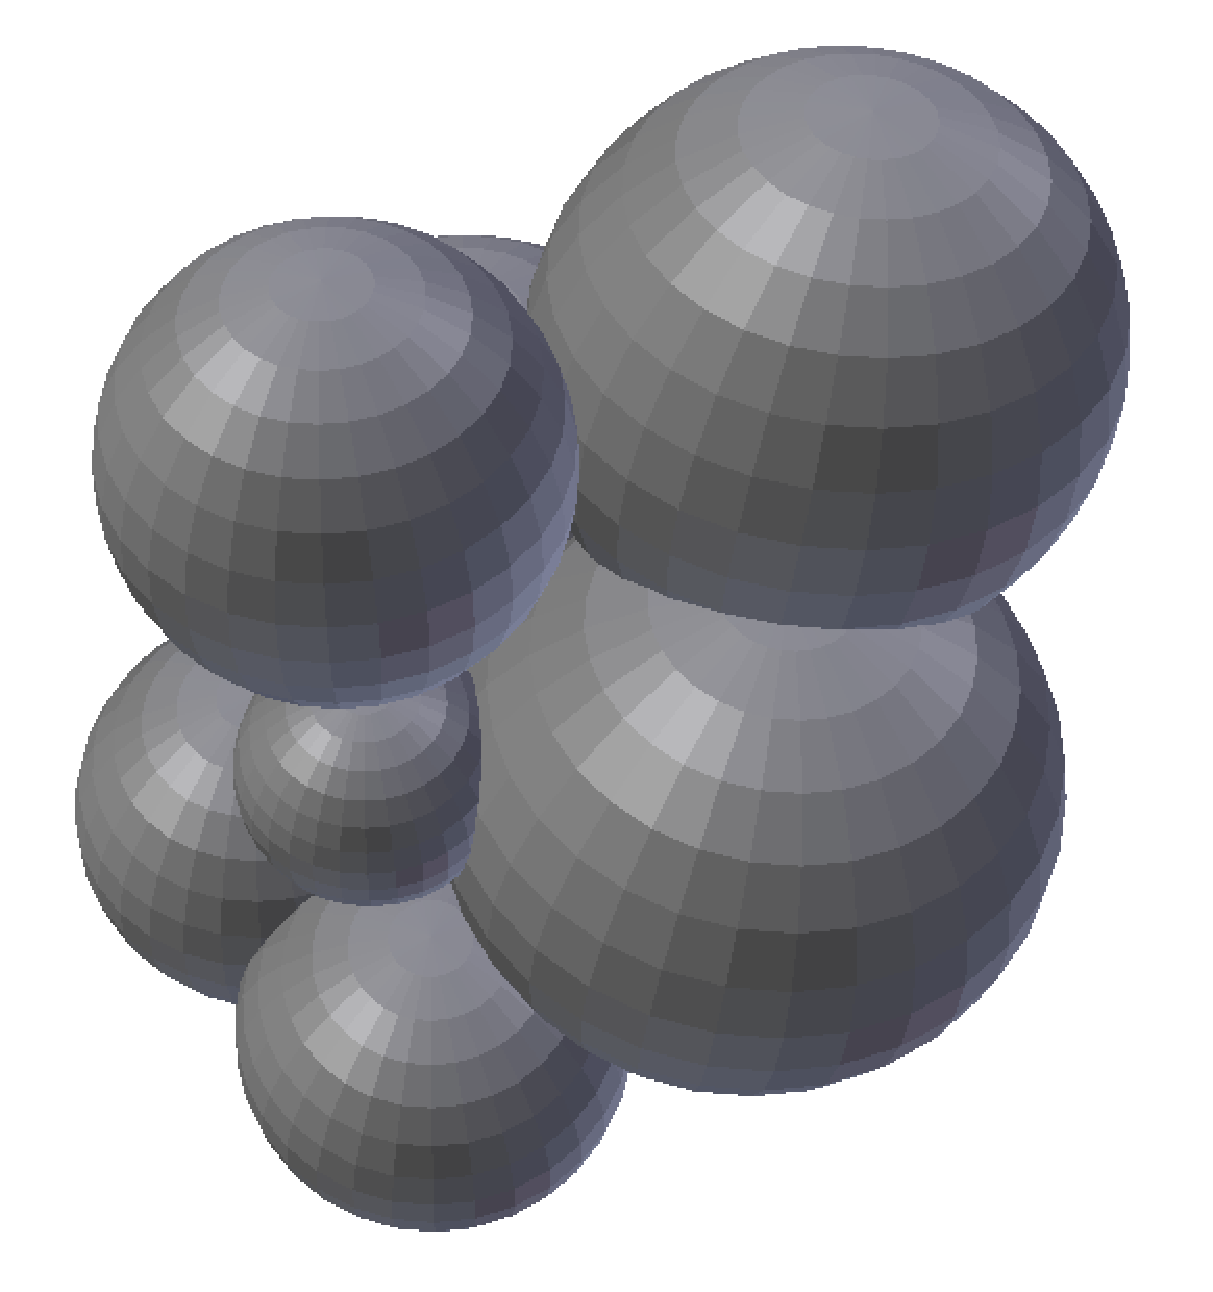
\includegraphics[width=0.8\linewidth]{figures/clunk}
	\end{minipage}%
	\begin{minipage}[t]{0.5\linewidth}
		\centering
		\includegraphics[width=0.8\linewidth]{figures/nointersect}
	\end{minipage}%
	\caption{Sample from geometric prior (left), whereas (right) is conditioned on no-intersection constraint}
	\label{fig:nointersect}
\end{figure}


\paragraph{Random Variables.} Probability models lie on top of probability
spaces. A probability space is a measure space $(\Omega, {\cal H}, {\cal P})$,
where ${\cal H}$ is a sigma algebra and ${\cal P}(\Omega) = 1$ \citep{ccinlar2011probability}. Random variables are
functions from the space $\Omega$ to a realization space ${\cal X}$. As a concrete
example the space $\Omega$ can be thought of as a hypercube, with ${\cal P}$ being
uniform over that hypercube. To build a normal random variable, we need a function
that maps from $\Omega \to \mathbb{R}$. If the underlying probability space is uniform, then
this function is the inverse cumulative distribution function of the normal.

A \emph{model} $\cM$ is a collection of random variables along with a probability space.
% To fully specify a model, we need both the measure space and the
% collection of random variables on which it acts.

\paragraph{Conditioning}

Conditioning a model creates a new model.
As an example consider a model $\cM$ with two
random variables $X_1$ and $X_2$ that both take real values. Conditioning
$\cM$ on $X_1 = 1$, defines a new model $\cM_{|A}$ based on limiting the measure space
$\Omega$ to the set $A = \{ \omega : X_1(\omega) = 1\}$.
The new model is defined on a new probability space
\begin{align}
	(\Omega \cap A, \{A \cap B, B \in {\cal H} \}, {\cal P} / {\cal P}(A))
\end{align}
with the same random variables $X_1$ and $X_2$.
Sampling from $\cM_{|A}$ produces
samples only where $X_1 = 1$

More generally, conditioning on any predicate $Y(\omega) = \lk(X_1(\omega), \dots, X_n(\omega))$
defines a new model defined exactly as above, where $A = \{\omega : \lk(X_1(\omega), \dots, X_n(\omega)) = 1\}$.
% This predicate may include a comparisonsuch as $X_i < X_j$, restrict deterministic function of variables in in the model such as $\exp(X_i) = 2$, or be a Boolean combination such as $(X_i < X_j) \lor \neg(\exp(X_i) = 2)$.
Sampling from $\cM_{|A}$ generates $(x_1, ..., x_n)$ where $\lk$ is true.

The general construction of new models might require conditioning
on sets of measure zero. This process can be made rigorous
via disintegration \citep{chang1997conditioning}. Disintegration can
be thought of as the reversal of building joint distributions through
product measure constructions.


% When building models with prior beliefs via conditioning, we would like
% the property that given an infinite collection of observations, the 
% posterior predictive distribution converges to true sampling distribution.
% To study this, consider a model with two random variables that are independent,
% $X_1$ is a function of $\omega_1$ and $X_2$ is a function of $\omega_2$. Suppose
% that the true sampling distribution has $X_1$ and $X_2$ positively correlated.
% For the prior beliefs to support positive correlations, we 
% could condition on a prior belief that $X_1$ and $X_2$ are close. However
% if the form of the closeness isn't controlled by a random variable, observing
% an arbitrary amount of data from the true distribution will not change
% the dependence between $X_1$ and $X_2$ in the model. 
% \begin{align*}
% X_j^*(\omega^*) = \sigma(f_\Beta(X_{j, 1}, ..., X_{j, n})) > b, \\
% \end{align*}
% Conditioning on $X_j^*$ produces a new set of models that have 
% dependence between . Knowledge is encoded in the prior distribution
% on $\Beta$. If $f_\Beta$ has priors over the true dependence between
% $X_{., 1},...,X_{., m}$, then this new model family will converge
% to the true underlying distribution.

% rr: TODO the above can me made into a proof

% \subsection{Bayesianism vs. Bayesian Computation}
% The way we 


% \section{Higher Order Random Variables}
% People often entertain beliefs about probability statements. For instance most people accept 
% trust expert-given odds that a particular sports team will win a tournament, 
% or politician will win an election, more than the odds of those given by non-experts.
% The apparent failure of probabilistic expressions to distinguish 
% between these cases led to alternative formalisms of uncertainty \citet{Shampher}, 
% but within the probabilistic framework both \citet{Pearl} and \citet{Hyberg} demonstrated 
% that such higher order distributions were induced from the original model, no new machinery was needed.

% As a concrete example of this, suppose we have a stochastic 
% dynamical system model of human blood glucose 
% controlled by some 
% parameters $\Theta$ with a prior. A priori we know that the average blood pressure 
% in a person lives in a physically plausible range $40-400$. A way to
% encode this would be to change the prior on the parameters $p(\Theta)$ 
% to so that any sample from that prior yields has average in the physically
% plausible range. This can be challenging because it requires a detailed
% understanding of the stochastic dynamical system. 

% Alternatively, we could try to take the conditioning approach from the
% previous section. But conditioning in the previous section required explicitly
% defined random variables, and while the average glucose is a random variable
% because the parameter $\Theta$ is random, it is not an explicit random variable.
% The scenario requires the ability to both define and condition on 
% probability distributions over either random variables or properties of 
% random variables (e.g. expectations).
% In this section we introduce the random conditional 
% distribution ($\randcond$) to support this task.

% \paragraph{The Random Conditional Distribution.}
% The random conditional distribution of $X$ given $\Theta$ -- which we denote $\rcd(X, \Theta)$ or $\rcdxy{X}{\Theta}$ -- is a random distribution: a random variable which takes values in the domain of random variables.
% Informally, $\rcdxy{X}{\Theta}$ is a function of $\omega$ that returns functions of $\omega$
% of the same type as $X$. Formally, $\rcd$ is a distribution over conditional random variables:

% % The primary mechanism for conditioning is $\cond$, which constructs conditional random variables:
% % \begin{definition}
% % Let $X:\Omega \to T$ be a random variable, $Y$ an indicator function, and $\conds{X}{Y}: \Omega_{|Y} \to T$ be a conditional random variable defined as: $X_{|Y}(\omega) = X(\omega)$.
% % $X_{|Y}$ is defined on a conditioned probability space $(\Omega, \Sigma, \mu_{|Y})$ where $\mu_{|Y}$ is a conditional measure: $
% % \mu_{|Y}(A) = \mu(A \cup Y^{-1}(\{1\})) / \mu(Y^{-1}(\{1\})$.
% % % That is, $\cond: (\Omega \to T) \times (\Omega \to \{0, 1\}) \to (\Omega \to T)$ is a operator that restricts the domain of $X$ to those inputs consistent with $Y$.
% % \end{definition}


% \begin{definition}The random conditional distribution of a random variable $X: \Omega \to T_1$ given $\Theta: \Omega \to T_2$ is a random variable $\rcdxy{X}{\Theta}: \Omega \to (\Omega \to T_1)$, defined as:
% \begin{equation}\label{eq:rcd}
% (\rcdxy{X}{\Theta})(\omega) = [\conds{X}{\Theta = \Theta(\omega)}]
% \end{equation}
% \end{definition}
% For example if $\Theta = \bern(0.4)$ and $X = \normal(\Theta, 1)$, then $\rcdxy{X}{\Theta}$ is a random distribution 
% whose domain comprises of two normal distributions $X_1 = \conds{\normal(\Theta, 1)}{\Theta = 1}$ and $X_2$.
% The probabilities of $X_1$ and $X_2$ with respect $\rcdxy{X}{\Theta}$ are determined by the prior probabilities of the different outcomes of $\Theta$: $P((\rcdxy{X}{\Theta}) = X_1) = 0.4$ and $P((\rcdxy{X}{\Theta}) = X_2) = 0.6$.

% A random conditional distribution is most useful in combination with other functions.
% Expectation is perhaps the most important example, which when composed with $\rcd$ produces conditional expectation.
% Restricting to real valued variables, expectation $E$ is a functional that maps a random variable to a real value
% (($\Omega \to \mathbb{R}) \to \mathbb{R}$).
% When $X$ is a real valued random variable, $\rcdxy{X}{\Theta}$ is not real valued, and hence not a valid argument to $E$.

% However, just as arithmetic operations such as $+$ and $-$ extend from the domain of numbers to the domain of random variable (pointwise $X + Y = \omega \mapsto X(\omega) + Y(\omega)$), $E$ extends from the domain of random variables to the domain of random variables over random variables in precisely the same way.
% % Since random variables are themselves functions, $E$ is an operator, functional or more generally a higher-order function.  
% % As described in section X a function with domain $T$ can be lifted to a functional of $T$-valued random variables.
% % $T$ is purposefully left abstract, because in addition to lifting functions defined on the reals etc, we can lift functions defined on random variables.
% % Expectation is a cannonical example of a random variable valued function, with type $E : (\Omega \to \mathbb{R}) \to \mathbb{R}$.
% That is, $\ee$ has a lifted counterpart $\lifted{\ee} = \lift(\ee)$ with type $\lifted{\ee} : (\Omega \to (\Omega \to \mathbb{R})) \to (\Omega \to \mathbb{R})$, which maps a distribution over real valued random variables to a distribution over real values (expectations).
% % $$
% % \lifted{\ee}(X)(\omega) = \mean{X(\omega)}
% % $$
% The operator $\rcd$ composed with $\ee$ constructs conditional expectation (with respect to a random variable $\Theta$):
% \begin{equation}
% \lmean{\rcdxy{X}{\Theta}} = \lmean{\omega \mapsto \conds{X}{\Theta = \Theta(\omega)}} 
%                     = \omega \mapsto \mean{\conds{X}{\Theta = \Theta(\omega)}}\\
% \end{equation}
% The final term $\omega \mapsto \mean{\conds{X}{\Theta = \Theta(\omega)}}$ matches the definition of
% conditional expectation
% with respect to a random variable $\mean{(X\mid \sigma (Y))(\omega)} = \mean{X \mid Y = Y(\omega))}$.
% That is the conditional expectation is a random variable with randomness provided by the conditioning set.

% Returning to the blood glucose example, we can build a model that respects the valid range
% of average blood glucose by taking the original model creating the conditional expected
% value of glucose $G$ with $\rcd$ and expectation of $\rcd$, then constructing a new model
% by conditioning the original on $G$ being in the physiologically possible range.

% \paragraph{Completeness.}Nested uses of $\rcd$ lead to a completeness result. State informally: 
% by repeatedly applying $\rcd$, any random function or functional in the original model
% can be constructed. Then by using conditioning to create new models from the previous 
% section, we can alter existing models to respect predicates on any random quantity in
% the model even if the random quantity is not an explicit random variable.
% % RR: TODO: The above could be a theorem


\section{Predicate Exchange}
To condition a model $\cM$ on a predicate $Y$ we develop Predicate Exchange, a likelihood-free inference procedure.  It is composed of two parts:
\begin{enumerate}
\item \textbf{Predicate Relaxation} constructs a relaxed predicate $\softv{Y}$ from $Y$. $\softv{Y}$ takes values in the unit interval $[0, 1]$ rather than $\{0, 1\}$.
$\softv{Y}$ is 1 iff $Y$ is 1, but otherwise takes nonzero values denoting the degree to which $Y$ is satisfied.
% The relaxation is parameterized by a temperature.
% Predicate relaxation allows us to apply likelihood based MCMC inference procedures.
\item  \textbf{Replica Exchange} is a Markov Chain Monte Carlo procedure that exploits temperature. The strength by which $\softv{Y}$ relaxes $Y$ is modulated by a temperature parameter $\alpha$, which trades off between accuracy and ease of inference.  By simulating several replicas of $\softv{Y}$ at different temperatures, replica exchange is able to draw exact samples. 
\end{enumerate}

\subsection{Predicate Relaxation}\label{predexchange}

A relaxed predicate $\softv{Y}$ approximates $Y$ in the sense that when viewed as a likelihood function on model parameters, $\softv{Y}$ has a broader support, assigning nonzero weights to parameter values which have zero weight under $Y$.
There are three desiderata which govern this approximation.
First, $\softv{Y}$ should have a temperature parameter $\alpha$ that controls the fidelity of the approximation. In particular, $\softv{Y}$ should converge to $Y$ as $\alpha \to 0$, and to a flat surface as $\alpha \to \infty$. Second, the fidelity of the approximation should vary monotonically with temperature. Third, $\softv{Y}$ should be consistent with $Y$ on 1. That is $Y(\omega) = 1$ iff $\softv{Y}(\omega) = 1$ at all temperatures.  


% The family of approximations of the predicate $Y$ is parameterized through a temperature $\alpha$ that controls the smoothness of the approximation. In particular, $\softv{Y}$ with $\alpha \to 0$ converges to $Y$ itself while increasing values of $\alpha$ yield smoother approximations eventually giving a flat surface when $\alpha \to \infty$. Moreover, the set of conditional samples $C(Y) = \{ \omega \in \Omega \text{ } | \text{ } Y(\omega) = 1 \}$ are assigned a value of $1$ in $\softv{Y}$ for all temperatures. 

% To construct a $\softv{Y}$ with such properties, we let $Y$ be the following predicate $a=b$ for standard Gaussians $a, b \sim \mathcal{N}(0, 1)$. We choose a distance
% $\rho(a, b)$ to indicate how close our sample is to $C(Y)$. To meet the desiderata
% of having $C(Y)$ be $1$ over the constraint set and to ensure the constraint becomes
% smoother with large $\alpha$, we use a function $k : [0, \infty] \to [0, 1]$ parameterized by $\alpha$ to wrap the distance $\rho(a, b)$. A simple choice for such a function is $k(d; \alpha) = e^{-d / \alpha}$ that provides the desired properties to $\softv{Y}$ (see Appendix). The formal definition of $\softv{Y}$ is as follows.

\begin{definition}
A function $\softv{Y} : \Omega \to [0, 1]$ parameterized by $\alpha \in [0, \infty)$ is a relaxation of a $Y: \Omega \to \{0, 1\}$ if:
\begin{enumerate}[label=(\roman*)]
	\label{def:temp}
	\item For all $\omega \in \Omega$, $\lim_{\alpha \to 0}\softv{Y}(\omega; \alpha) = Y(\omega)$.
	\item For all $\omega \in \Omega$, $\lim_{\alpha \to \infty}\softv{Y}(\omega; \alpha) = 1$.

    \item For all $\alpha$, $\softv{Y}(\omega; \alpha) = 1$ iff $Y(\omega) = 1$.
    \item The entropy $H(\softv{Y}(\omega; \alpha))$ (which characterizes the fidelity of the approximation ) is an increasing function of $\alpha$.\footnote
    {By compactness, it is integrable for all $\alpha$, when $\Omega$ has finite dimension}
\end{enumerate}
\end{definition}


The construction of $\softv{Y}$ from $Y$ (Section \ref{implement}) substitutes primitive predicates (equality, inequalities and logical operators) in the model with soft predicates.  Soft predicates rely on a notion of distance; the degree to which a predicate is satisfied is a measure of closeness in a metric space. 
For example if $x$ and $y$ are real values, then $x \soft{=} y$ is defined as $k_\alpha(\rho(x, y))$ where $\rho$ is a distance function and $k_\alpha$ is a relaxation kernel paramterized by temperature $\alpha$.
In general, we use $\soft{p}$ to denote a relaxation of a predicate $p$.
A relaxation kernel maps distances to values in $[0, 1]$, and ensures that $\softv{Y}$ adheres to the outlined criteria.
There are several possible kernels but we restrict our attention to the squared exponentional kernel:
\begin{equation}
k_{\alpha}(r) = \exp\left(-\frac{r^2}{\alpha}\right)
\end{equation}

\paragraph{Distance}The distance $\rho$ depends on the realization spaces of random variables.
For canonical spaces such as $\mathbb{R}$ and $\mathbb{N}$ we default to Euclidean distances. 
For example, $x \soft{=} y$ is then defined as $\exp(\norm{x - y}/\alpha)$.
For elements of composite structure taking with a product typem $x, y \in \mathbb{T}_1 \times \cdots \times \mathbb{T}_n$, by default $\rho$ takes a mean $\rho(x, y) = (1/n)\sum^n_{i=1}\rho(x_i, y_i)$.

A soft inequality such as $x \soft{>} y$ is function of the amount by which $x$ must be increased (or $y$ decreased) until $x > y$ is true.
This is the distance between $x$ and the interval $[y, \infty]$, where the distance between a point and any interval $[a, b]$ is the smallest distance between $x$ and any element in $[a, b]$, and therefore 0 if $x \in [a, b]$:
\begin{equation}
\rho(x, [a, b]) =
\begin{cases}
  a - b & \text{ if } x < a\\
  x - b & \text{ if } x < b\\
  0              & \text{otherwise}
\end{cases}
\end{equation}

The optimal degree of satisfaction $\soft{\lk}_{\inf}(m)$ of a realization $m = (x_1, \cdots x_n)$ of a model is then the smallest distance between that realization and any point in the constraint set, i.e.,
\begin{equation}
\soft{\lk}_{\inf}(m) = \rho(m, A)
\end{equation}
where $A = \{(x_1, \dots, x_n) \mid \lk(x_1, \dots, x_n) = 1\}$, and $\rho(x, A) = \inf \left\{\rho(x, a) \mid a \in A\right\}$
As shown in the Section \ref{implement}, $\soft{\lk}_{\inf}$ can be difficult to compute.

  % \begin{center}
  % \begin{tabular}{ c |  c | c }
  %   \hline		
  %   $x \soft{=} y$ & $x \soft{>} y$ & $x \soft{<} y$  \\
  %   $k_\alpha(\rho(x, y))$ & $k_\alpha(\rho(x, [y, \infty]))$ & $k_\alpha(\rho(x, [-\infty, y]))$ \\
  %   \hline  
  % \end{tabular}
  % \end{center}


\begin{figure}\label{softpreds}
  \begin{align*}
x \soft{=} y &= k_\alpha(\rho(x, y))\\
x \soft{>} y &= k_\alpha(\rho(x, [y, \infty]))\\
% x \soft{<} y &= k_\alpha(\rho(x, [-\infty, y]))\\
x \soft{<} y &= k_\alpha(\rho(y, [-\infty, x]))\\
a \soft{\land} b &= \max(a, b)\\
a \soft{\lor} b &= \min(a, b)
  \end{align*}
\caption{Soft Primitive Predicates}
\end{figure}

\paragraph{Negation}
Negation is a necessary component of a Boolean algebra, but its relaxation introduces complications.
To illustrate, Figure \ref{negationimg} (a) shows $x \soft{>} 0$ as a function of $x$.
In continuous logics \cite{kimmig2012short}, the negation of $a \in [0, 1]$ is $1 - a$.
However, as shown in Figure \ref{negationimg} (b), this violates criteria (iii) of predicate relaxation; there are values which satisfy the hard predicate $\neg(x > 0)$ which do take a value of 1 in $1 - (x \soft{>} 0)$.

\begin{figure}
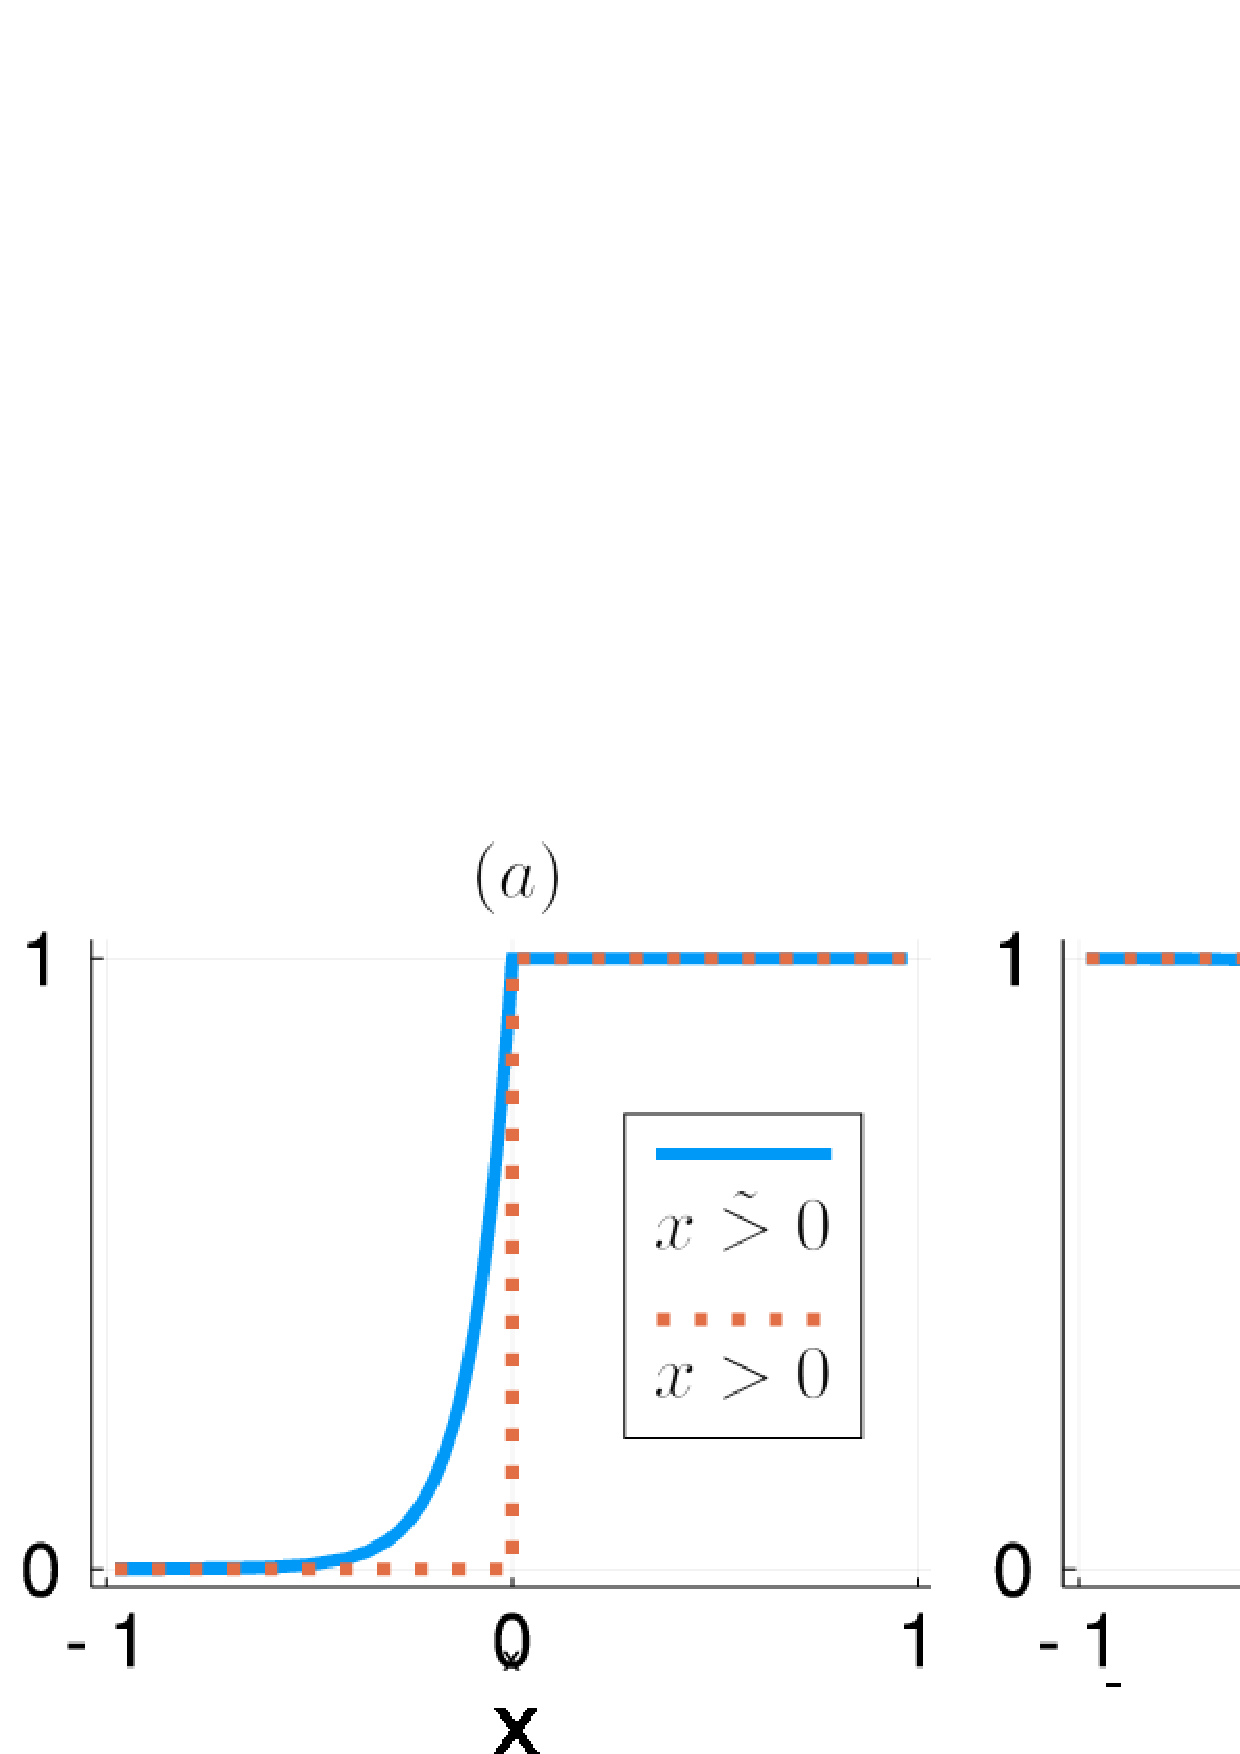
\includegraphics[width=\linewidth]{negation.pdf}
\caption{Soft predicates as function of $x$.  In all figures the blue line denotes the soft predicate, while the red line denotes the predicate to approximate.}\label{negationimg}
\end{figure}


The problem of negation arises because $\softv{Y}$ is consistent with $Y$ at 1 but not at 0.
In other words, $\softv{Y}$ is a one-sided approximation.
To overcome this challenge for models where negation is used, a two-sided relaxed predicate yields a pair $(a_0, a_1)$, where $a_0, a_0 \in [0, 1]$.
$a_1$ preserves consistency with $Y$ on $1$, just as before, while $a_0$ preserves consistency with $\neg Y$ on $1$ (or equivalently $Y$ on 0).
For example if $x \dsoft{>} 0 = (a_0, a_1)$, then as a function of $x$, $a_0$ and $a_1$ correspond to Figure \ref{negationimg} (a) and (c) respectively.

A complete two-sided soft logic is shown in Figure \ref{softw}.
Observe that soft negation simply swaps the elements of $(a_0, a_1)$ to yield $(a_1, a_0)$.
Although a two-sided predicate has two components, for the sake of conditioning we are still concerned only with the true side $a_1$ in the pair $(a_0, a_1)$.

% \begin{definition}
% The function $\softv{Y} : \Omega \to [0, 1]^2$ parameterized by $\alpha \in [0, \infty)$ is a two-sided relaxation of a $Y: \Omega \to \{0, 1\}$ if:
% \begin{enumerate}[label=(\roman*)]
% 	\label{def:temp}
% 	\item For all $\omega \in \Omega$, $\lim_{\alpha \to 0}\softv{Y}(\omega; \alpha) = (\neg Y(\omega), Y(\omega))$.
% 	\item For all $\omega \in \Omega$, $\lim_{\alpha \to \infty}\softv{Y}(\omega; \alpha) = (0, 1)$.

%     \item For all $\alpha$, $\softv{Y}(\omega; \alpha) = 1$ iff $Y(\omega) = 1$.
%     \item The entropy $H(\softv{Y}(\omega; \alpha))$ (which characterizes the fidelity of the approximation ) is an increasing function of $\alpha$.\footnote
%     {By compactness, it is integrable for all $\alpha$, when $\Omega$ has finite dimension}
% \end{enumerate}
% \end{definition}


\begin{figure}\label{softw}
\begin{align*}
x \dsoft{=} y &= (\text{if } x = y  \text{ then } \alpha \text{ else } 1, k_\alpha(\rho(x, y)))\\
x \dsoft{>} y &= (k_\alpha(\rho(x, [-\infty, y])), k_\alpha(\rho(x, [y, \infty])))\\
x \dsoft{<} y &= (k_\alpha(\rho(y, [x, \infty])), k_\alpha(\rho(y, [-\infty, x])))\\
(a_0, a_1) \dsoft{\land} (b_0, b_1) &= (a_0 \soft{\land} b_0, a_1 \soft{\land} b_1)\\
(a_0, a_1) \dsoft{\lor} (b_0, b_1) &= (a_0 \soft{\lor} b_0, a_1 \soft{\lor} b_1)\\
\dsoft{\neg}(a_0, a_1) &= (a_1, a_0)
\end{align*}
\caption{Two sided soft primitive predicates}
\end{figure}

% \begin{center}
% \begin{tabular}{ l | c | r }
%   % \hline		
%   $(a_0, a_1) \soft{\land} (b_0, b_1)$ & $(a_0, a_1) \soft{\lor} (b_0, b_1)$ & $\neg(a_0, a_1)$ \\
%   $(a_0, a_1) \soft{\land} (b_0, b_1)$ & $(a_0, a_1) \soft{\lor} (b_0, b_1)$ & $\neg(a_0, a_1)$ \\
%   % \hline  
% \end{tabular}
% \end{center}



\subsection{Approximate Markov Chain Monte Carlo}
A relaxed predicate can serve as an approximate likelihood, and as a result is amenable to likelihood based inference methods such as Markov Chain Monte Carlo.
MCMC algorithms require a function $f$ that is proportional to the the target density.
In Bayesian inference this is the posterior, dictated by Bayes' theorem as the product of the likelihood and the prior.
Approximate inference using relaxed predicates takes a similar form.

Let $\cM = (X_1, \dots, X_n)$ be a model, $Y$ be a predicate that conditions $\cM$, and  $\softv{Y}(\omega) = \softv{\lk}(X_1(\omega), ..., X_n(\omega))$ be a relaxation of $Y$.
% % Random variables in $\cM$ may be exogenous or endogenous in the sense that
% % given values for exogenous variables, the values of endogenous are determined.
% % For example $X = \mathcal{N}(0,1)$ is exogenous while $Y = X^2$ is endogenous.
% % Inference need only take place on exogenous random variables.
% Both $Y$ and $\softv{Y}$ are random variables, and hence map from the sample space $\Omega$;
% for convenience we define a soft predicate $\softv{\lk}$ as a function of its parameters (other random variables in the model) rather than the sample space.
% That is, let $\softv{Y}(\omega) = \softv{\lk}(X_1(\omega), ..., X_n(\omega))$, where $X_i \in \cM$.
Assuming a prior density $p$, the approximate posterior $f$ is the product:
\begin{equation}
f(m) = p(m) \cdot \softv{\lk}(m)
\end{equation}
$\softv{\lk}$ down weights parameter values which violate $Y$ by the degree to which they violate it. 
This is modulated by the temperature $\alpha$ used in the  relaxation kernels which constitute $\softv{\lk}$.
At maximum temperature $\softv{\lk}$ has no effect, and the approximate posterior $f$ is equal to the prior $p$.
At zero temperature, $f$ recovers the true posterior since parameter values which violate the condition are given zero weight.

For illustration, let $\cM = (\mu, X_1, X_2)$ be a model where $\mu = \mathcal{N}(0, 1), Y = \mathcal{N}(\mu, 1)$, $X_2 = X_1^2$ and $\cM$ be conditioned on $X_2 = 1$.
Since $X_2$ is a deterministic function of $X$, we can exclude it for inference.
The approximate posterior is shown at different temperatures in Figure \ref{temppost} and defined as:
\begin{equation}\label{approxposterior}
f(x, y) = \mathcal{N}_{0,1}(x) \cdot \mathcal{N}_{0,1}(y) \cdot k(x + y, 0) 
\end{equation}

\begin{figure}\label{temppost}
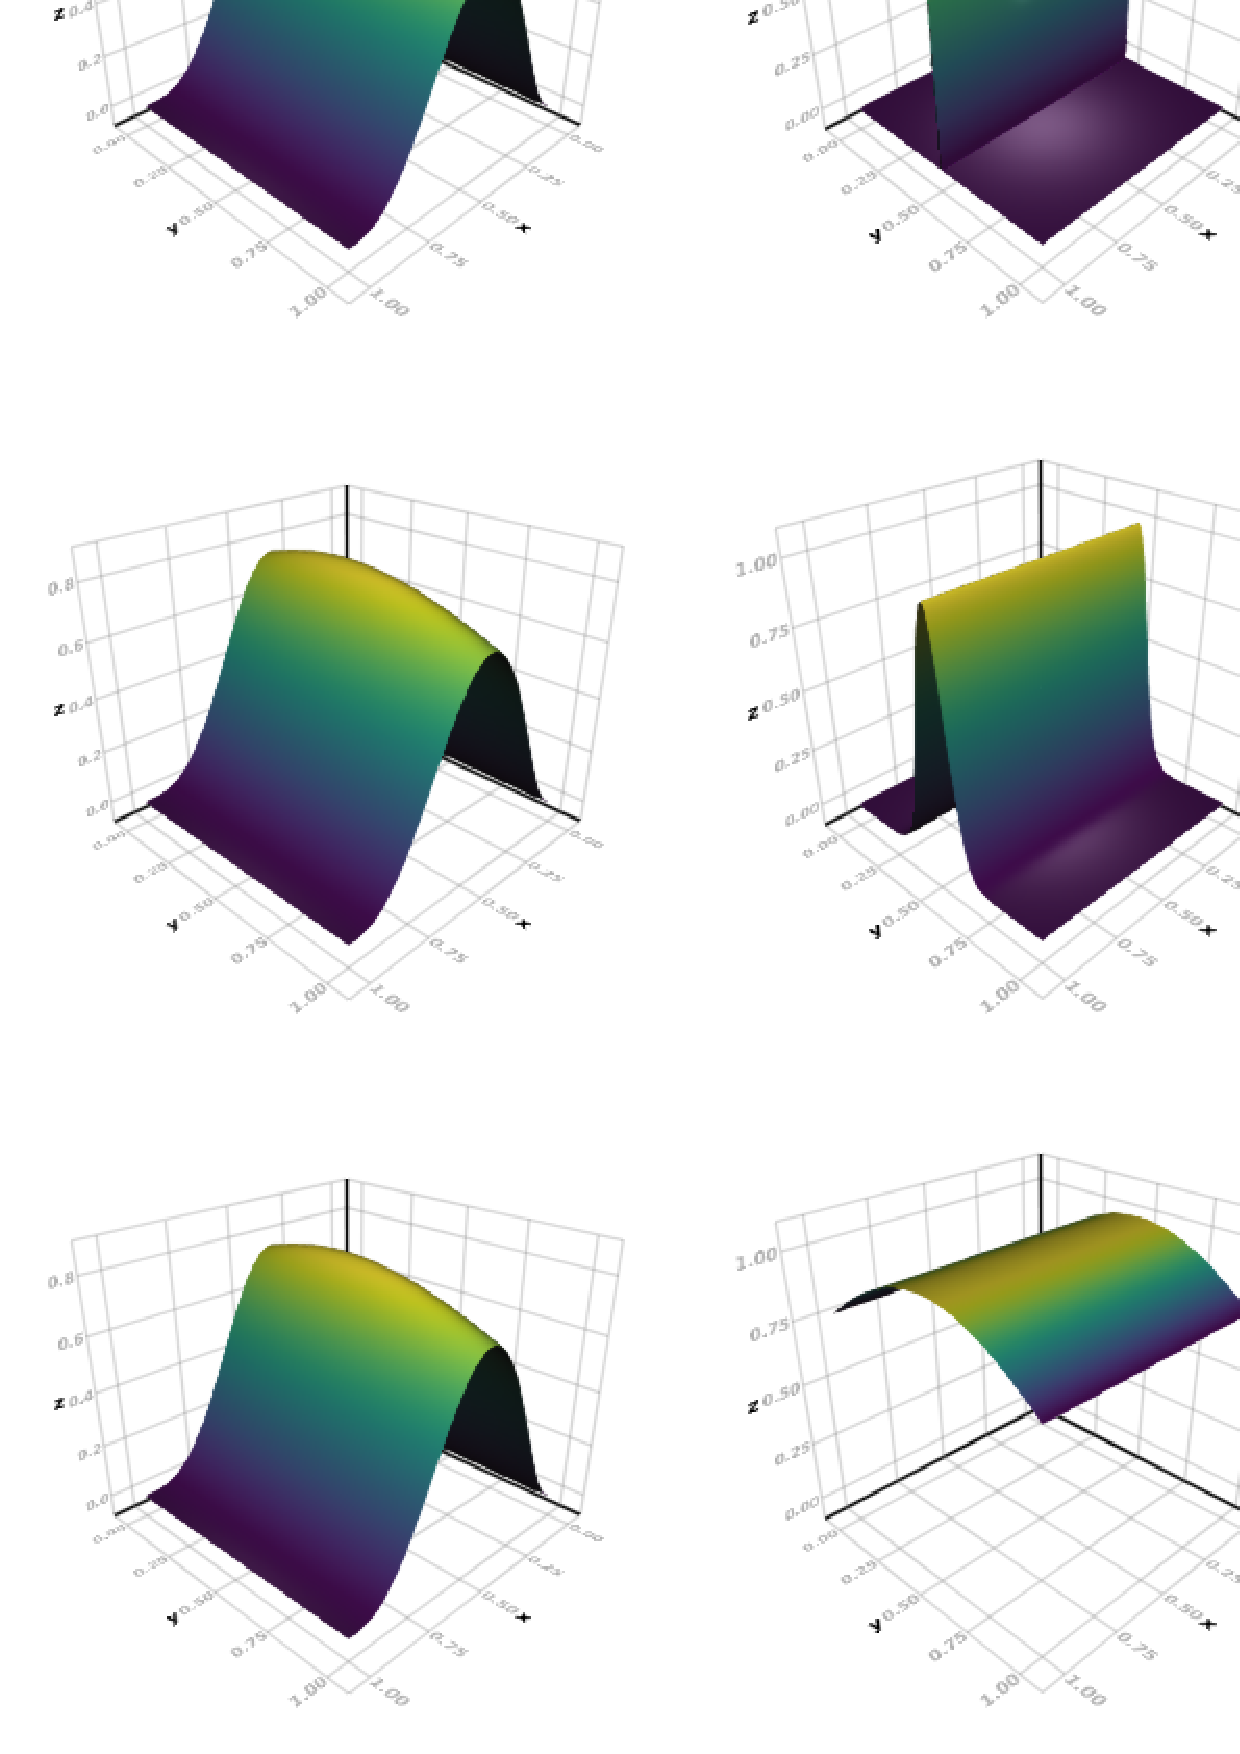
\includegraphics[width=\linewidth]{approxpost.png}
\caption{Approximate Posterior at varying temperatures}
\end{figure}

The temperature parameter trades off between tractability of inference and the fidelity of the approximation.
Too high and $\softv{Y}$ will diverge too greatly from $Y$   . Too low and convergence will be slow.
% Several temperatre methods for controlling temperature exist such as simulated annealing \citep{kirkpatrick1983optimization} and Adiabatic Monte Carlo \citep{betancourt2014adiabatic}.
We augment replica exchange \citep{swendsen1986replica}, which combines information from several chains to sample more effectively, which an accept/reject phase, to sample from the unrelaxed model.

\subsection{Replica Exchange}\label{replicaexchange}
Replica exchange simulates $M$ replicas at different temperatures, and uses a Metropolis-Hastings update to  periodically swap the temperatures of chains.
Given w.l.g two parallel chains simulating targets $f_{\alpha_1}(x)$, $f_{\alpha_2}(y)$ where $f_{\alpha_i}$ is an approximate posterior function at temperature $\alpha_i$.
Assuming independence, they follow a joint target $f_{\alpha_1, \alpha_2}(x,y) = f_{\alpha_1}(x)f_{\alpha_2}(y)$.
Replica exchange swaps states between the two chains while preserving the joint target.
That is, we propose a swap of $x$ and $y$ to move from $(x, y)$ to $(x^\star,y^\star)$, where $x^\star=y$ and $y^\star=x$.
Swapping states is equivalent to swapping predicates, which motivates the name predicate exchange.
The swap is accepted with probability $\min(1, A)$ where:
\begin{equation}
A = \frac{f_{\alpha_1, \alpha_2}(x^\star,y^\star)}{f_{\alpha_1, \alpha_2}(x,y)} = \frac{f_{\alpha_1, \alpha_2}(y,x)}{f_{\alpha_1, \alpha_2}(x,y)} = \frac{f_{\alpha_1}(y)f_{\alpha_2}(x)}{f_{\alpha_1}(x)f_{\alpha_2}(y)}
\end{equation}

For exact inference, states which violate the constraint are rejected.
Unlike conventional replica exchange which draws samples only from the zero-temperature chain, we accept states from any chains so long as $f_{\alpha_i}(x) = 1$.

Replica exchange has a number of hyper-parameters: the number of parallel chains, the corresponding temperatures, the swapping schedule.
Several good practices are outlined in Following \cite{earl2005parallel}.  In practice, we logarithmically space $\alpha$ between a lower and upper bound (e.g., $\alpha_1 = 10^{-5}$, $\alpha_M = 10^5$), and swap states of chains that are adjacent in temperature ($\alpha_1$ with $\alpha_2$, $\alpha_2$ with $\alpha_3$, etc) periodically.


\paragraph{Balancing Different Constraints}
The scales of variables effect their influence on
the conditional distribution at a fixed temperature.
For example consider two pairs of variables, where
the first pair is ten times larger than the second.
Conditioning on a greater than constraint on both
pairs of variables is well defined. However,
a softening of both constraints would have 
a much larger change in the energy function over
a standard deviation change in pairs of variables.
To mitigate this issue, Omega tries enforce equality
in magnitude between all basic predicates at each temperature.
% rr: zenna can you add the basic predicates
To accomplish this, consider the case of two 
softened predicates $k_1$ and $k_2$. For the
energy function, Omega introduces a weight
for all but the first constraint, in this
case $k_2$ in the energy function gets replaces
by $\gamma_2 k_2$. The weight $\gamma_2$ should
ensure that $\gamma_2 k_2$ has the same
magnitude effect as $k_1$ on the energy
function:
\begin{align*}
E_{p_{\alpha, \gamma_2}}[k_1] = E_{p_{\alpha, \gamma_2}}[\gamma_2 k_2] 
\end{align*}
% Does such a gamma_2 always exist? Maybe rewrite it as
% an optimization problem over gamma to enforce a solution?
In practice, we set $\gamma_2$ using an exponential moving
average of the $k_1$ values over the $k_2$ values.

% This scenario closely resembles the reparameterization trick \citep{Kingma:2014, rezende2014stochastic} where one resorts to include all the uncertainty of a random variable $z$ in a simple, easy-to-sample, parameter-free noise source such as $\epsilon \sim \mathcal{N}(\mathbf{0}, I)$. The actual random variable $z$ is then obtained through a parametric transformation of the noise, $z = f(\epsilon; \theta)$. Both methods separate the 
% uncertainty of a random variable from the deterministic transformation that results in a complex density. However, in the reparameterization trick the noise source is constant and controlled while the parametric transformation is meant to infer the structure of the resulting random variable. Conversely, our forward model -- deterministic transformation -- is constant and controlled, hence we simply transfer our inference problem to a much simpler space of $\Omega$.

% Predicate Exchange has a connection to approximate Bayesian computation (ABC) methods~\citep{beaumont2002approximate} in that ABC methods 
% sample using a distance function to induce a data likelihood. Our method differs in that conditionals can be any predicate not just
% one for an observed random variable.
% Finally for inference, with the soft predicates we define, we
% can use modern likelihood-free variational inference algorithms
% that construct an approximation to a conditional with only samples
% from the joint and samples from the conditional approximation~\citep{tran2017hierarchical}.


\section{Implementation}\label{implement}

% Our approach to inference is not black-box.
% It requires a transformation of the model.
% This can be realized in a number of ways.
% To formalize this we introduce a very simple language for describing probabilistic models.
% Following this, we demonstrate how these principle can be incorporated into existing languages.


% \subsection{A Minimal Language}{\label{minilang}}


% \begin{figure}[t]
% 	\begin{align*}
% 		\text { model term }  &  & \enspace m ::=               & e ; \cond f \\
% 		\text { standard term }  &  & \enspace e ::=               & e ; e \mid v \sim f\\
% 		\text { standard term }  &  & \enspace f ::=               & p \mid f \textrm{ bop }f \mid\textrm{ op } f \mid \\
% 		\text { standard term }  &  & \enspace f ::=               & \text{ if } t_1 \text{ then } t_2 \text{ else } t_3 \\
% 		\text { binary op }      &  & \enspace \textrm{bop} ::=    & + \mid - \mid / \mid * \mid \land \mid \lor \mid > \mid < \mid \\
% 		\text { unary op }       &  & \enspace \textrm{uop} ::=    & \lnot                                                          \\
% 		\text { primitive dist } &  & \enspace p ::= \bern(f) \mid & \unif(f, f) \mid N(f, f) \mid                                  \\
% 	\end{align*}
% 	\caption{Abstract Syntax}
% 	\label{syntax}
% \end{figure}

% Figure \ref{Syntax} describes the abstract syntax of our language.
% The language closey resembles statistical notation.
% One difference is that conditions are stated at the end of each model in a single statement $\cond$.

% Here is an example.

% \begin{align*}
% 	x \sim   & \unif(0, 1)           \\
% 	y \sim   & \unif(0, 1)           \\
% 	\cond \; & (x = y) \land (x > 3) \\
% \end{align*}

% \subsubsection{Semantics}\label{semantics}
% \newcommand{\sem}[1]{\llbracket #1 \rrbracket}
% Here we define a semantics denotationally.
% The denotation $\sem{t}$ of a term $t$ is a value in a semantic domain corresponding to an \omegalang{} type, such as a Boolean, real number, or random variable.
% Primitive 


% \subsection{Syntactic Predicate Relaxation}

% The transformation from the original model to a relaxed model is straight forward.
% Algorithm substitutes X accepts as input the abstract syntax

% \begin{figure}[t]
% 	\begin{align*}
% 		\text { model term }  &  & \enspace m ::=               & e ; \cond f \\
% 		\text { standard term }  &  & \enspace e ::=               & e ; e \mid v \sim f\\
% 		\text { standard term }  &  & \enspace f ::=               & p \mid f \textrm{ bop }f \mid\textrm{ op } f \mid \\
% 		\text { standard term }  &  & \enspace f ::=               & \text{ if } t_1 \text{ then } t_2 \text{ else } t_3 \\
% 		\text { binary op }      &  & \enspace \textrm{bop} ::=    & + \mid - \mid / \mid * \mid \land \mid \lor \mid > \mid < \mid \\
% 		\text { unary op }       &  & \enspace \textrm{uop} ::=    & \lnot                                                          \\
% 		\text { primitive dist } &  & \enspace p ::= \bern(f) \mid & \unif(f, f) \mid N(f, f) \mid                                  \\
% 	\end{align*}
% 	\caption{Abstract Syntax}
% 	\label{syntax}
% \end{figure}

% \begin{align*}
% 	x \sim \unif(0, 1)              \\
% 	y \sim \unif(0, 1)              \\
% 	ll \sim x =_s y \land_s x >_s 3 \\
% \end{align*}

% \subsection{A Lightweight Implementation}\label{rng}

In this section we describe a generic, lightweight implementation of predicate exchange.
Our approach closely mirrors \citep{wingate2011lightweight, milch20071} in the sense that it provides a language independent layer that can be implemented on top of existing programming languages and modeling formalisms.
Our objective is to twofold: (i) to compute the prior term $p$, approximate likelihood term $\lk$, and approximate posterior term $f$ (Equation \ref{approxposterior}) from an arbitrary program $\pi$, and (ii) to perform Replica Exchange MCMC to sample from this posterior.

A program $\pi$ can be an arbitrary composition of deterministic and stochastic procedures, but all stochastic elements must come from a set of known \emph{elementary random primitives}, or ERPs.
ERPs correspond to primitive parametric distribution families, such as the uniform or normal distribution.
Let $\mathcal{T}$ be a set of ERP types.
Each type $\tau \in \mathcal{T}$ must support (i) evaluation of $p_\tau(x \mid \theta_1, ..., \theta_n)$: the conditional probability of $x$ as a function of its parameters, and (ii) sampling from the distribution.
Concretely, a conditioned program $\pi$ is a any program that includes:

\begin{enumerate}
  \item $\textrm{rand}(\tau, n, \theta_1, ...,\theta_n)$ returns a random sample from $p_\tau(x \mid \theta_1, ..., \theta_n)$.
  \item $\cond(y)$ throws an error if $y \in \{0, 1\}$ is 0, and otherwise allows simulation to resume with no effect.
\end{enumerate}



\subsection{Tracked Soft Execution}
The prior term $p$ is computed automatically as the product of independent random choices in the program. 
That is, let $\pi_{k \mid x_1, ..., x_{k-1}}$ be the k'th ERP encountered in while executing $\pi$, $x_k$ be the value it takes, and $x$ denote the set of all values of all ERPs constructed in the simulation of $\pi$.
The probability $p(x)$ is the product:
\begin{equation}\label{productprob}
p(x) = \prod_{k=1}^K p_\tau(x_k \mid \theta_1,..., \theta_n )
\end{equation}
Crucially, the parameters $\theta_1,..,\theta_n$ for each random variable may be fixed values or depend on values of other random variables in $\pi$.

Predicate exchange relies on $\textrm{softexecute}$
(Algorithm \ref{alg:softexecute}), which formalizes the soft execution of a program $\pi$ at temperature $\alpha$, in the context of dictionary $\mathbb{D}$.
A dictionary $\mathbb{D}$ is a mutable mapping from a set of names to values.
In the context of a particular dictionary, the simulation of a program is deterministic.
This allows the simulation of $\pi$ to be modulated by controlling the elements of $\mathbb{D}$.
Concretely, $\textrm{softexecute}$ simulates $\pi$ but redefines the definition of several operators, with $\lk_\pi$ and $p_\pi$ in global scope and both initialized at $1$:

\begin{enumerate}
  \item $\textrm{rand}(\tau, n, \theta_1, ...\theta_n)$ returns $\mathbb{D}(n)$ if exists, otherwise samples from $p_\tau(x \mid \theta_1, ..., \theta_n)$ and updates $\mathbb{D}(n)$ with this value.  Also, in compliance with Equation \ref{productprob}, $p_\pi$ is updated with conditional density. 
  \item $a \text{ op } b$ and $\textrm{op } a$ for $\textrm{op} \in \{>, <, =, \land, \lor, \neg\}$ are replaced with the softened counter-parts $\soft{\textrm{ op }} \in \{\soft{>}, \soft{<}, \soft{=}, \soft{\land}, \soft{\lor}, \soft{\neg}\}$.
  \item $\cond(y)$ updates $\lk_\pi$ with $\lk_\pi \land y$ where $y \in [0,1]$ due to soft primitive operators.  
\end{enumerate}

The return value is a real value denoting the approximate posterior $f$, which are a function of the dictionary $\mathbb{D}$.

\begin{algorithm}[tb]
  \caption{Soft Execution: $\textrm{softexecute}(\pi, \alpha, \mathbb{D})$}
  \label{alg:softexecute}
\begin{algorithmic}
\STATE {\bfseries Input:} program $\pi$, temperature $\alpha$, dictionary $\mathbb{D}$
\STATE Initialize $\lk_\pi = 1, p_\pi = 1$
\STATE Simulate $\pi$, intercept statements any statement $s$, wbere:   
\IF{$s = \textrm{rand}(\tau, n, \theta_1, ..., \theta_n)$}
 \IF{$n \in \mathbb{D}$}
   \STATE $x = \mathbb{D}(n)$
 \ELSE
   \STATE $x = $ sample from $p_\tau(x \mid \theta_1, ..., \theta_n)$
   \STATE Update dictionary: $\mathbb{D}(n) = x$
 \ENDIF
 \STATE $p_\pi = p_\pi \cdot p_\tau(x \mid \theta_1, ..., \theta_m)$
 \ELSIF{$s = \cond(\lk')$}
   \STATE $\lk_\pi = \lk_\pi \cdot \lk_\pi'$
 \ENDIF
\STATE {\bfseries Return:} $p_\pi \cdot \lk_\pi$
%    \ENDFOR
%    \UNTIL{$noChange$ is $true$}
\end{algorithmic}
\end{algorithm}

\subsection{Replica Exchange}

Predicate exchange (Algorithm \ref{alg:predexchange}) performs replica exchange using $\textrm{softexectute}$ as an approximate posterior.
It takes as input an mcmc algorithm, which is expected to return a sequence of dictionaries which capture the Markov Chain.
We assume a dictionary contains all the information of latent variables of interest, either explicitly or derivable with the simulator $\pi$. 

For finite dimensional continuous models we use the No U-Turn Sampler \cite{hoffman2014no} -- a variant of Hamiltonion Monte Carlo -- as the within-chain MCMC procedure. 
% For other models we use.
Both are elaborated on in the implementation section.

\begin{algorithm}[tb]
  \caption{Predicate Exchange}
  \label{alg:predexchange}
\begin{algorithmic}
\STATE {\bfseries Input:} program $\pi$, temperatures $\alpha_1, ...,\alpha_m$, nsamples $n$
\STATE {\bfseries Input:} mcmc, $q$ number within samples
\STATE Initialize $\mathcal{D} = $ empty collection of dictionarys
\STATE Initialize $\mathbb{D}_1,...,\mathbb{D}_m$ empty dictionarys
\REPEAT
  \FOR{$i=1$ {\bfseries to} $m$}
    \STATE { $\mathbb{D}_1,...,\mathbb{D}_q = $ draw $q$ mcmc samples at temp $\alpha_i$}
    \IF {i = 1}
      \STATE append $\mathbb{D}_1,...,\mathbb{D}_m$ to $\mathcal{D}$
    \ENDIF
  \ENDFOR
  \FOR{$i = m$ {\bfseries to} $2$}
    \STATE $j = i - 1$
    \STATE $p = \frac{a}{b}$
    \IF{$p > $}
      \STATE swap $\alpha_i$ with $\alpha_j$
    \ENDIF
  \ENDFOR
\UNTIL{$forever$}
\STATE {\bfseries Return:} $\mathcal{D}$
\end{algorithmic}
\end{algorithm}


\section{Experiments}\label{experiments}

\paragraph{Experimental Setup}Replica exchange requires a within chain MCMC algorithm.
For finite dimensional continuous models we use the No U-Turn Sampler \cite{hoffman2014no}, a variant of Hamiltonion Monte Carlo (HMC).
We use reverse-mode automatic differentiation \cite{griewank2008evaluating} to compute the negative log gradient of $f$, which is required for HMC.
For other models we use standard Metropolis Hastings by defining proposals on elements in the dictionary.
In particular we use the single site Metropolis Hastings (SSMH) \cite{wingate2011lightweight} which modifies a single random variable at a time.

Replica exchange has a number of hyper-parameters: the number of parallel chains, the corresponding temperatures, the swapping schedule.
Several good practices are outlined in \cite{earl2005parallel}.  In practice, we logarithmically space $\alpha$ between a lower and upper bound (e.g., $\log_{10}(\alpha_1) = 5$ to $\log_{10}(\alpha_M) = -5$), and swap states of chains that are adjacent in temperature ($\alpha_1$ with $\alpha_2$, $\alpha_2$ with $\alpha_3$, etc) periodically.


\paragraph{Small Models}
In Figure \ref{fig:density} we use conditioning to truncate a normal distribution. Figure  \ref{gridn} shows histograms of samples from a uniform prior  $[-1, 1]^2$ conditioned on a variety of predicates.  While simple, these examples can be challenging due to discontinuities in the approximate posterior.

% \begin{figure}[!htb]
% 	\centering
% 	\includegraphics[width=0.9\linewidth]{swapmats}
% 	\caption{Analysis of Replica Exchange}
% 	\label{swapmats}
% \end{figure}	


\begin{figure}[!htb]
	\centering
	\includegraphics[width=0.9\linewidth]{gx2}
	\caption{Samples from models using different procedures.  Each model is $x,y \sim \unif(-1,1)$ conditioned on (i) $x \soft{=} y$, (ii) $|x| \soft{>} |y|$, (iii) $x^2 \soft{=} y^2$ and (iv) $\sin(kx)\cos(kx) \soft{>} 0.9999$.
	Inference procedures are: Single Site Metropolis Hastings (SSMH), Hamiltonian Monte Carlo (HMC), and Predicate-Exchange (PE) using HMC and SSMH within chain.}
	\label{gridn}
\end{figure}	

\begin{figure}[!htb]
\centering
\textbf{Truncated Normal through Conditioning}\par\medskip
\includegraphics[width=0.5\linewidth,trim={0.5cm, .3cm, .5cm, .1cm}, clip]{truncated}
\includegraphics[width=0.44\linewidth,trim={2.0cm, .2cm, 2cm, 1.2cm}, clip]{swapmats}
% \fbox{\includegraphics[width=0.44\linewidth,trim={2.0cm, .2cm, 2cm, 1.2cm}, clip]{swapmats}}

% \begin{minipage}{0.45\linewidth}
% \includegraphics[width=\linewidth]{truncated}
% \end{minipage}%
% \begin{minipage}{0.45\linewidth}
% 	%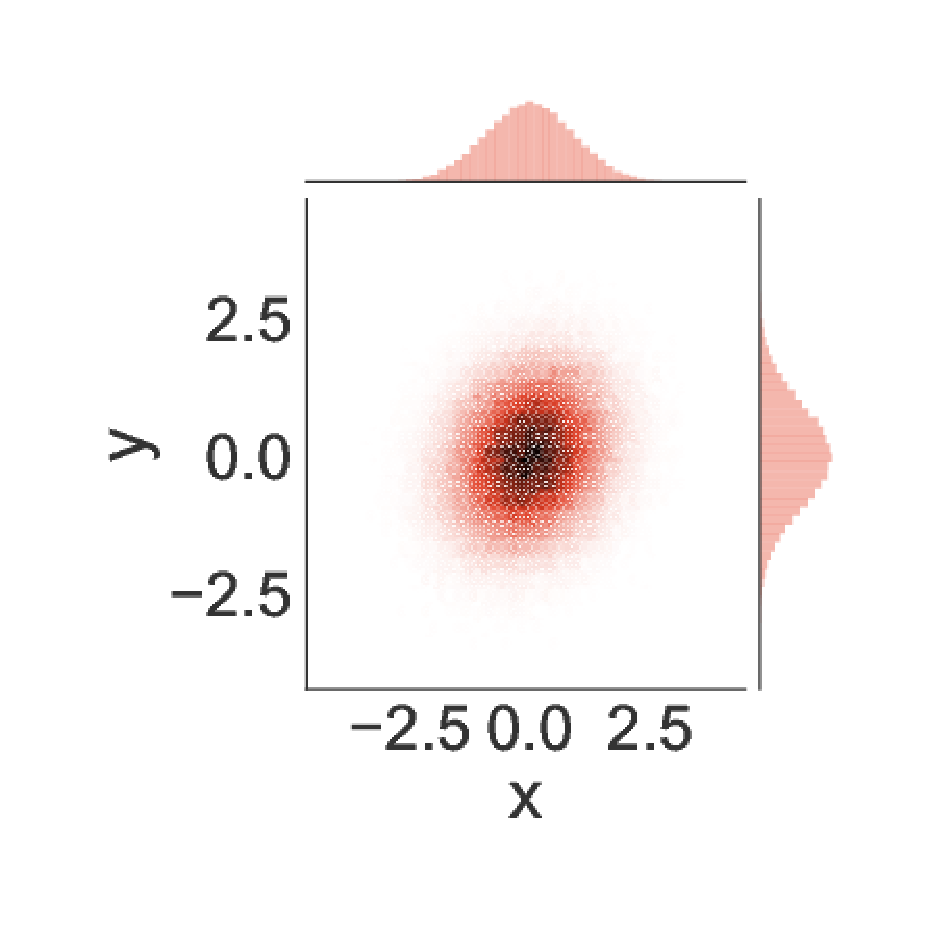
\includegraphics[width=.16\linewidth, trim={1.7cm, 1.6cm, 1.3cm, 1.5cm}, clip]{0-1}
% 	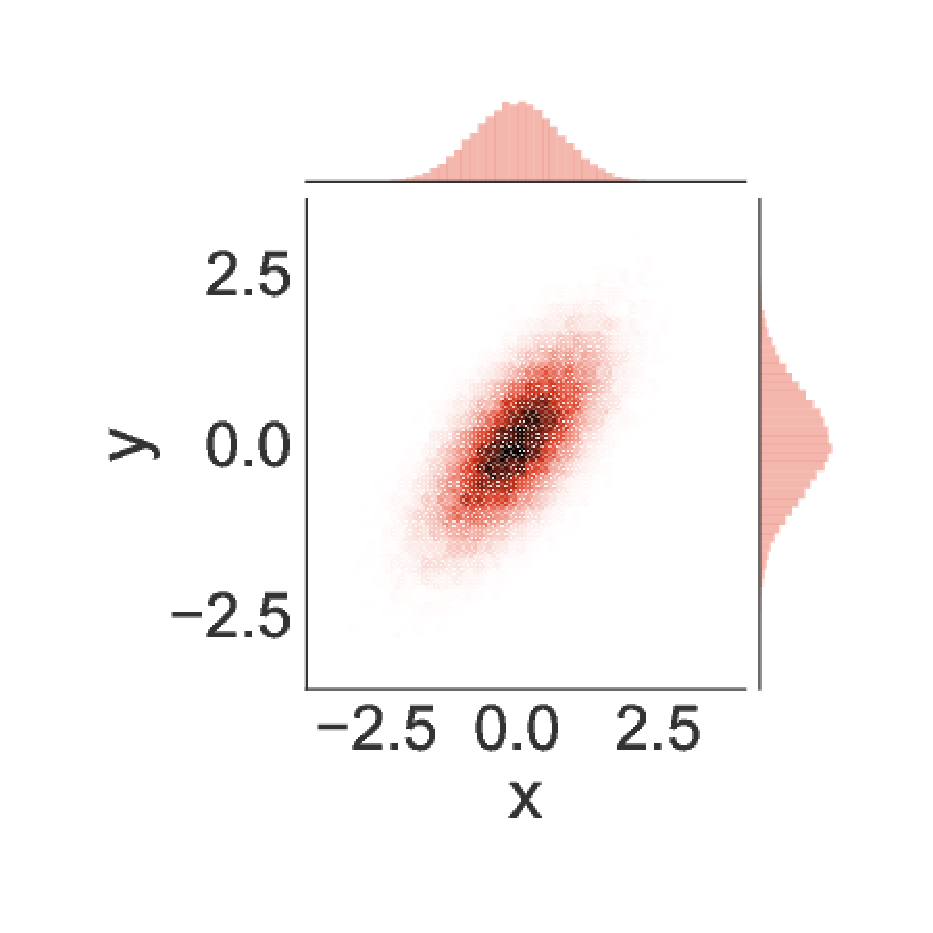
\includegraphics[width=.45\linewidth, trim={1.7cm, 1.6cm, 1.3cm, 1.5cm}, clip]{1-0}
% 	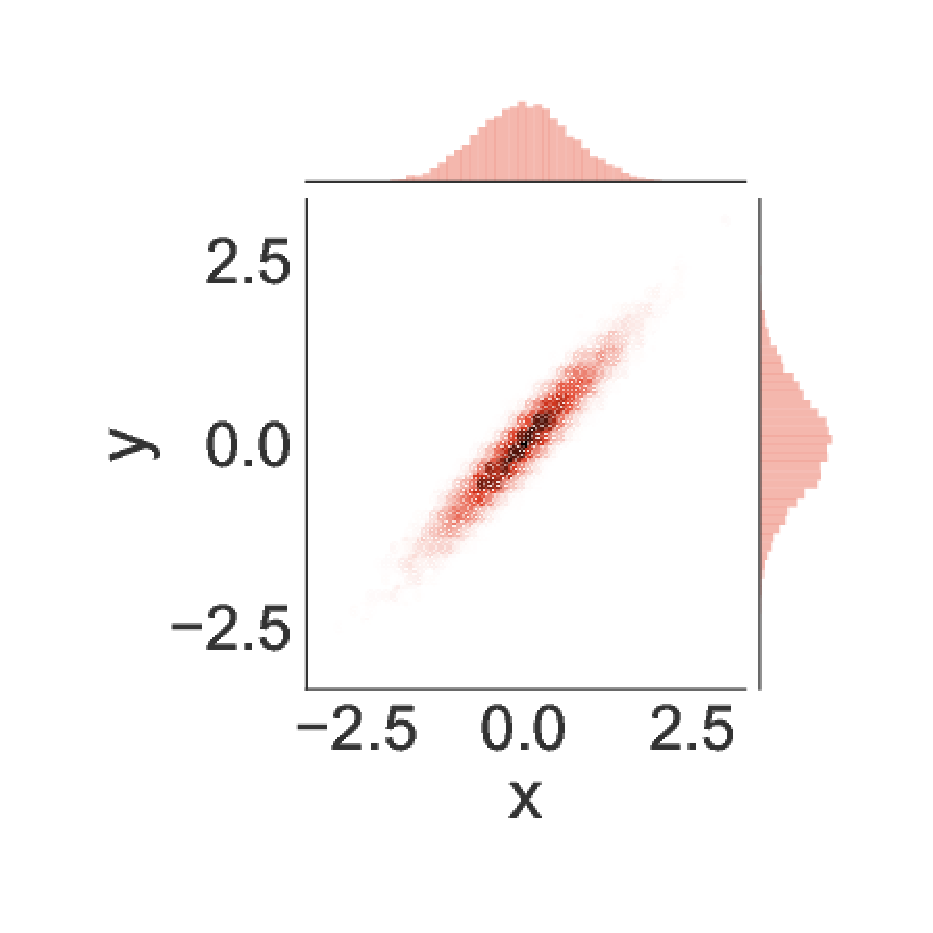
\includegraphics[width=.45\linewidth, trim={1.7cm, 1.6cm, 1.3cm, 1.5cm}, clip]{10-0}
	
% 	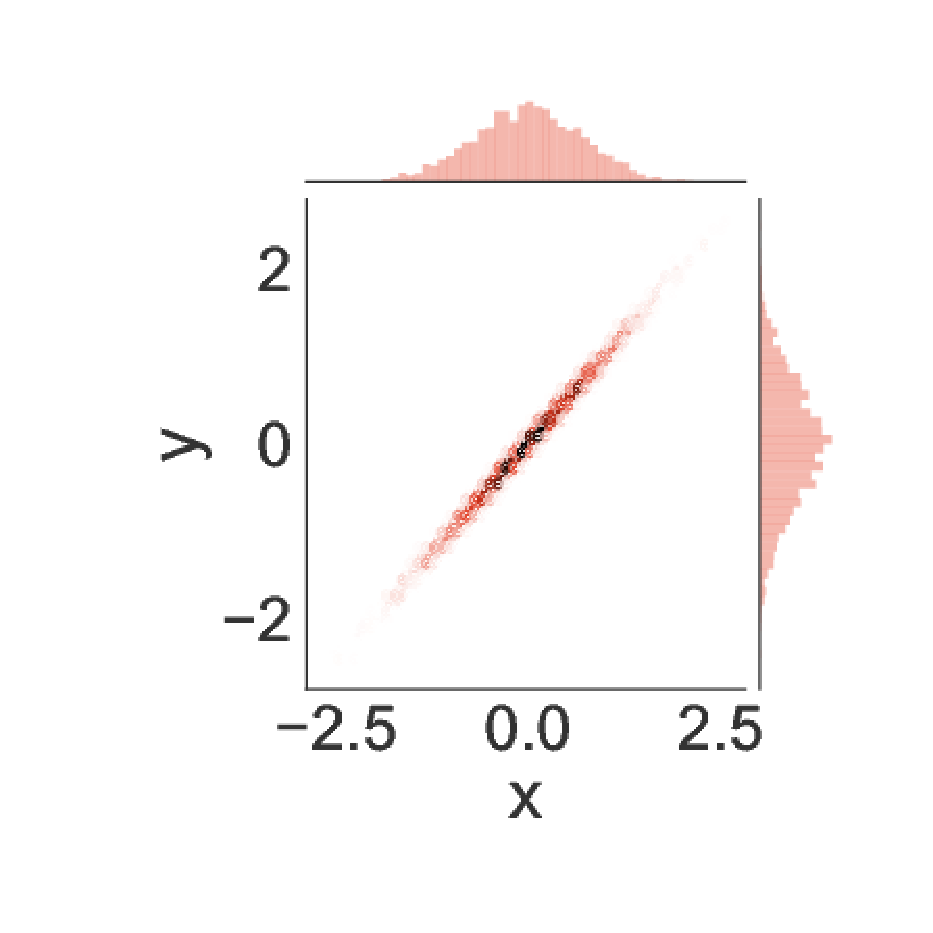
\includegraphics[width=.45\linewidth, trim={1.7cm, 1.6cm, 1.3cm, 1.5cm}, clip]{100-0}
% 	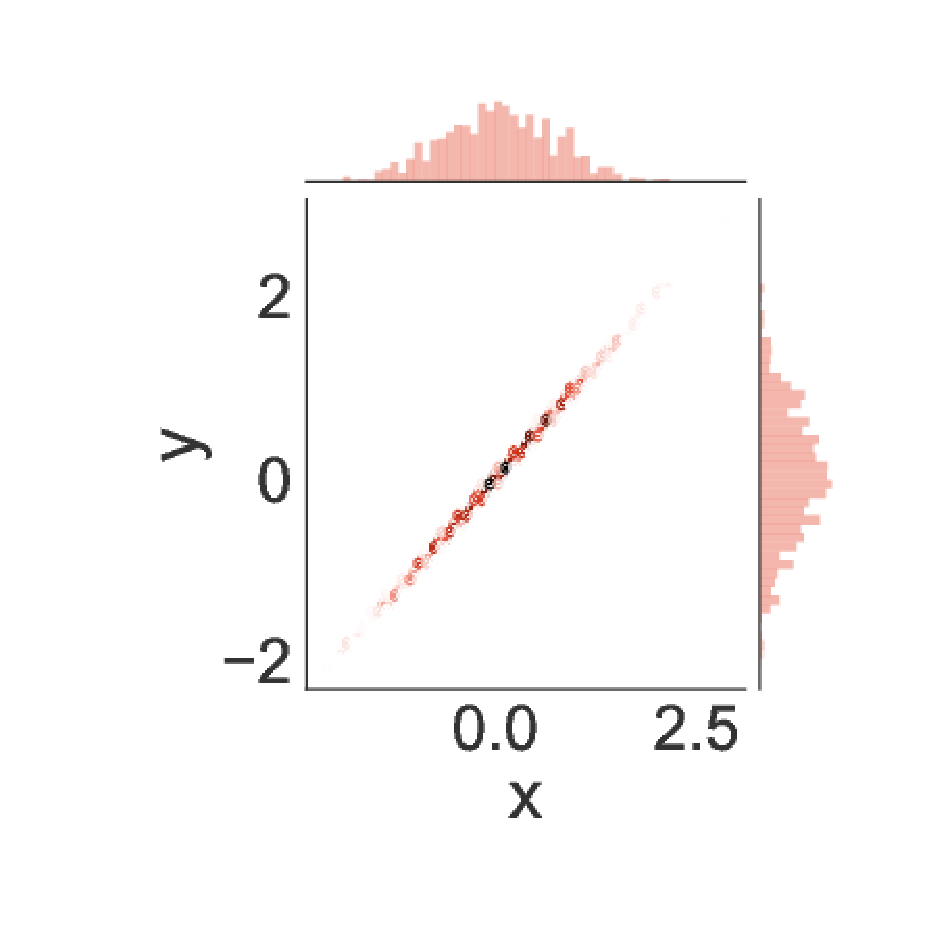
\includegraphics[width=.45\linewidth, trim={1.7cm, 1.6cm, 1.3cm, 1.5cm}, clip]{1000-0}				
	
% %	\fbox{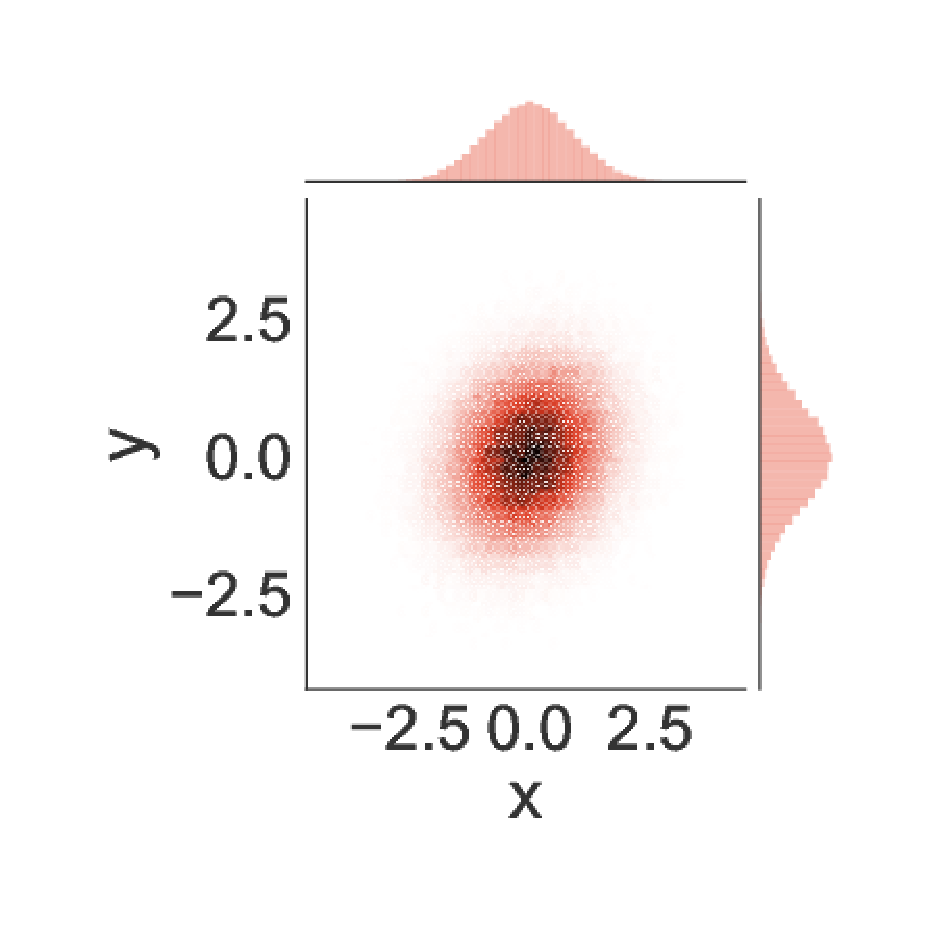
\includegraphics[width=.16\linewidth, trim={1.7cm, 1.6cm, 1.3cm, 1.5cm}, clip]{0-1}}
% %	\fbox{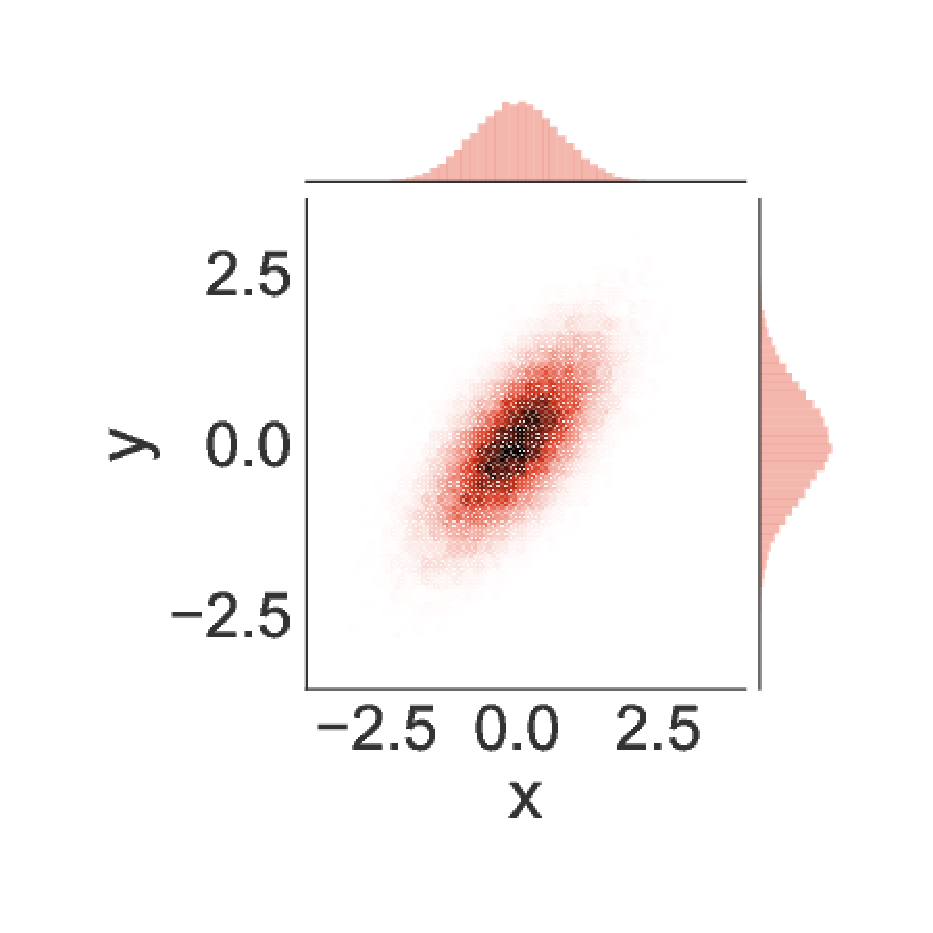
\includegraphics[width=.16\linewidth, trim={1.7cm, 1.6cm, 1.3cm, 1.5cm}, clip]{1-0}}
% %	\fbox{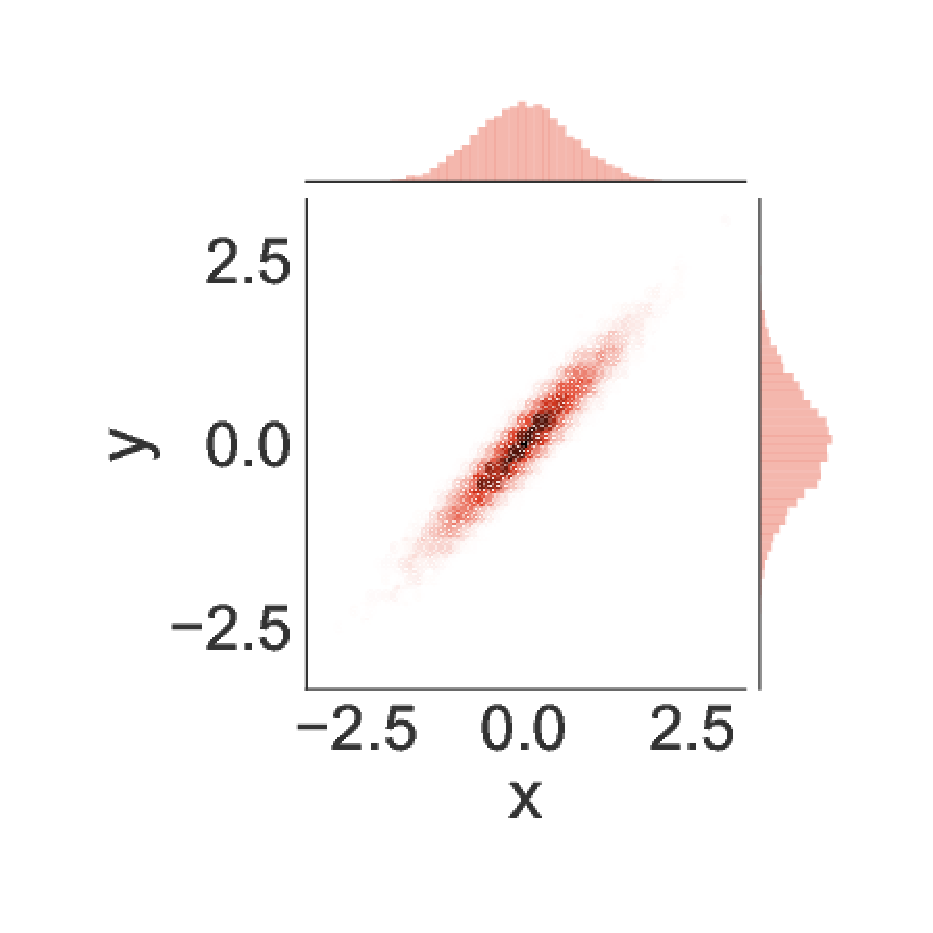
\includegraphics[width=.16\linewidth, trim={1.7cm, 1.6cm, 1.3cm, 1.5cm}, clip]{10-0}}
% %	\fbox{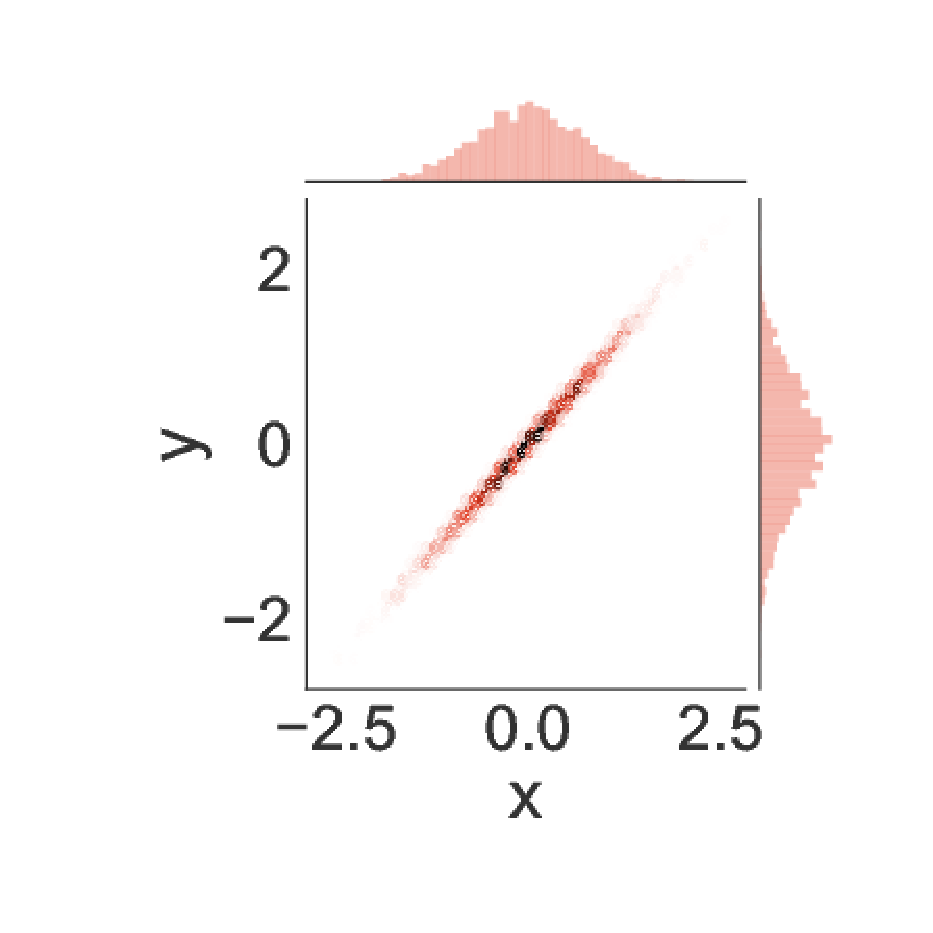
\includegraphics[width=.16\linewidth, trim={1.7cm, 1.6cm, 1.3cm, 1.5cm}, clip]{100-0}}
% %	\fbox{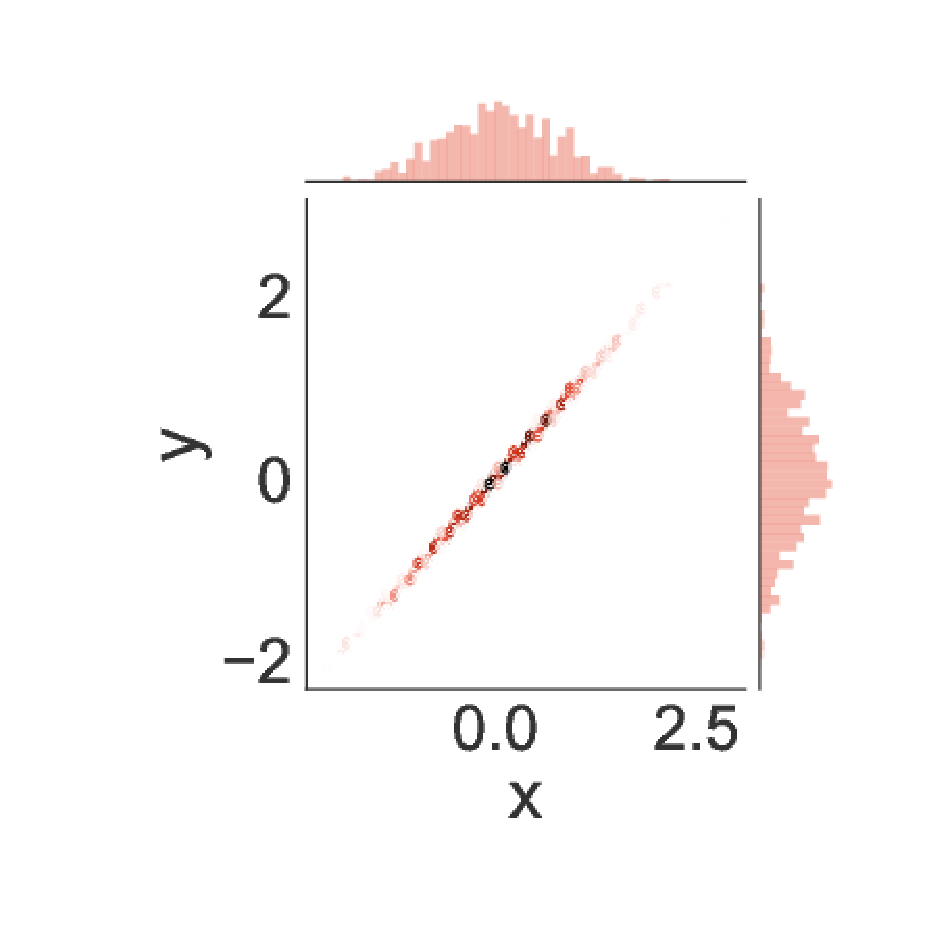
\includegraphics[width=.16\linewidth, trim={1.7cm, 1.6cm, 1.3cm, 1.5cm}, clip]{1000-0}}				
% 	\end{minipage}
	\caption{Left: Kernel density estimation from samples of Gaussian truncated to $[0, 1]$ through conditioning. Shown at different temperatures. Right: transitions between different temperatures of replica exchange.  For each matrix, value in row $i$ and column $j$ is the fraction of times replica exchange swapped a state at temperature $i$ to temperature $j$.  Temperature is lowest at 4 and increases exponentially to 1.  Clockwise, starting top-left: transition counts are accumulated for the first, second, third and fourth quarters of simulation.}
	\label{fig:density}
\end{figure}



\paragraph{Inverse Ray Tracing}
In this example we sample from a posterior distribution over scenes conditioned on an observed rendering.  A scene $s$ is a set of $n \sim \textrm{poisson}(\lambda = 3)$ spheres.
A sphere is parameterized by color, reflectance, emission color, transparency, radius and position, all with a uniform prior.
Let $r$ be a ray tracing function that maps scenes to image, $i_{obs}$ be an observed image, and $\textrm{nointersect}$ be a predicate that maps a scene to 1 iff any spheres intersect.
The prior $s$ is conditioned on the conjunction of the inverse rendering and the no-intersection constraints:

\begin{equation}
(r(s) = i_{obs}) \land \textrm{nointersect}(s)
\end{equation}

Figure \ref{fig:invrtmcmc} visualizes conditional samples.
% \begin{figure}
% 	\centering
% 	\includegraphics[width=0.9\linewidth]{invg2.pdf}
% 	\includegraphics[width=0.9\linewidth]{invgb.pdf}
% 	% \includegraphics[width=0.9\linewidth]{lvstime.pdf}
% 	% \includegraphics[width=0.9\linewidth]{Hausdorf.pdf}
% 	\caption{ Samples from inverse graphics.}
% 	\label{fig:invrtmcmc}
% \end{figure}

\begin{figure}
	\centering
	\includegraphics[width=0.9\linewidth]{jampy2.pdf}
	\caption{Inverse rendering with and without no-intersection constraints.  Top row: raytraced scenes.  Bottom row: red pixels denote the existence of an intersection between spheres at that point.  (middle) and (right) scenes are samples from posterior over scenes having observed image on left.  The observed scene has no intersections.  Without the no-intersection condition (right), intersections occur.  Conditioning on intersection eliminates intersections (middle).}
	\label{fig:invrtmcmc}
\end{figure}


\paragraph{Glucose Model}
Type 2 diabetes is a prevalent and costly condition.
Keeping blood glucose within normal limits helps prevent the
long-term complications of Type 2 diabetes like diabetic neuropathy and diabetic retinopathy \citep{brownlee2006glycemic}. Models to predict the trajectories of blood glucose aid in keeping glucose within
normal limits \citep{zeevi2015personalized}. Traditional models have been built from compositions of differential equations \citep{albers2017personalized,levine2017offline} whose parameters are estimated separately for each patient. An alternative approach would be to use a flexible sequence model like an RNN. The problem with this approach is that an RNN can extrapolate to glucose values incompatible with human physiology. This is especially a problem where we have patients with only a few blood glucose measurements. To build an RNN model that respects physiology, we condition on it.

We compare the independent RNN model to the one with declarative knowledge on a second patient from Physionet \citep{moody2001physionet}.
Figure \ref{fig:rnn-samples} plots the results performed on more than 300 pairs of patients.
We see that the conditional model simulates
more realistic glucose dynamics for the patient 
with only a short observed time-series.

% 1) Glucose modeling is a real problem \cite, \cite. 
% 2) Models have focused on ODEs \cite \cite 
% 3) Alternative is to use RNN 
% 4) RNN can produce nonsense result 
% 5) Conditioning helps


% Taken from the supplement in \cite{albers}

% \paragraph{A constrained model of glucose dynamic}
% Take glucose measurements across time $t$ from 
% N patients indexed by $i$: $x_{t,i}$.
% We model the glucose time series for each patient can be modeled independently using a recurrent neural network: 
% \begin{align*}
% W_i &\sim N(0, I) \\
% x_{t, i} &= f(x_{t-1, i}, W).
% \end{align*}
% This model treats all patients as independent. However,
% we have extra knowledge in that the average-across-time glucose levels will be similar across patients. Expressing this kind of knowledge by tying the parameters $W_i, W_j$ is a challenge because the structure of the recurrence function alters how $W$ controls the average outputs. In this sense, we would like to condition on the distance between conditional expectations being close for some distance $d$,
% \begin{align*}
% 	E\left(\sum_{t=1}^{T_i} E[x_{t, i} \,|\, W_i], \sum_{t=1}^{T_j} E[x_{t, j} \,|\, W_j]\right) < \delta_E,
% \end{align*}
% for all patient pairs $i, j$. Additionally, we would like to make the series smooth controlling for their variance:
% \begin{align*}
% 	d_{Var}\left(\sum_{t=1}^{T_i} Var[x_{t, i} \,|\, W_i], \sum_{t=1}^{T_j} Var[x_{t, j} \,|\, W_j]\right) < \delta_{Var},
% \end{align*}
%  We compare the independent model
% to the one with the conditional model learned on five patients. 
% We see that the conditional model simulates more realistic glucose dynamics for the patient with only a short observed time-series.

\begin{figure}[!htb]
	\centering
    %\fbox{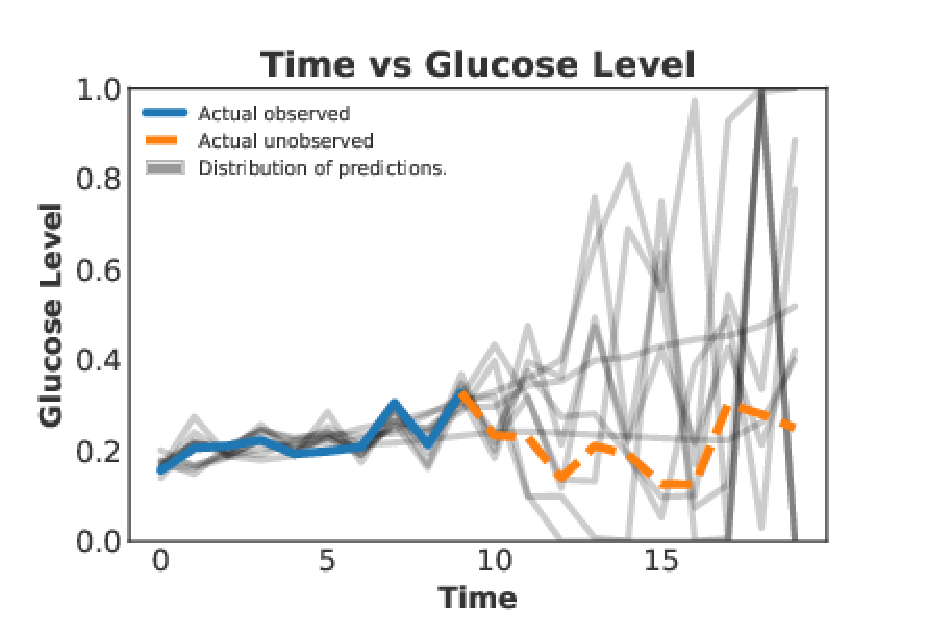
\includegraphics[width=0.30\linewidth, trim={1.cm, 0.1cm, 1.3cm, .5cm}, clip]{rnnsamples-no-tie-py}}
	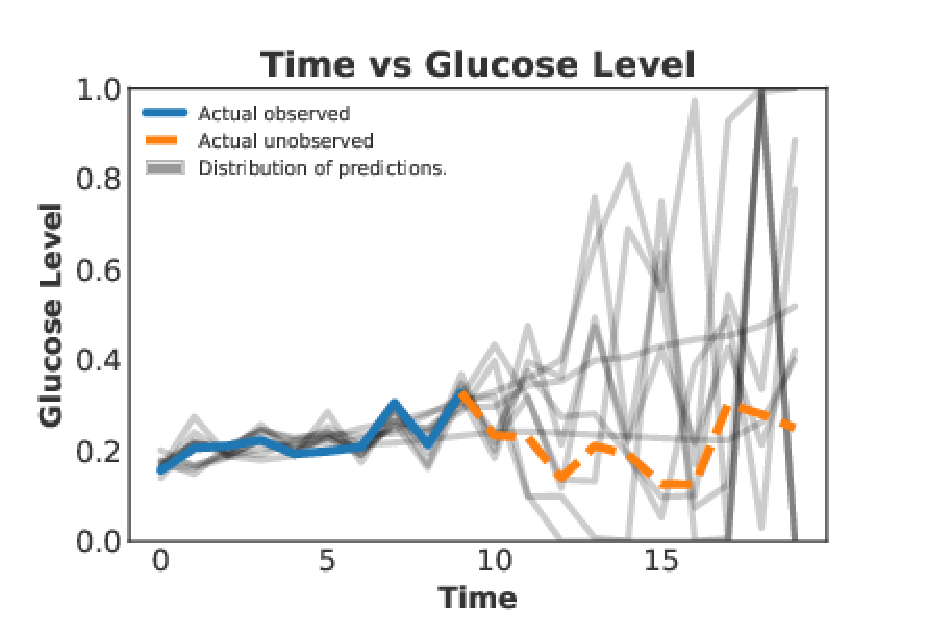
\includegraphics[width=0.7\linewidth, trim={1.cm, 0.1cm, 1.3cm, .5cm}, clip]{rnnsamples-no-tie-py}
	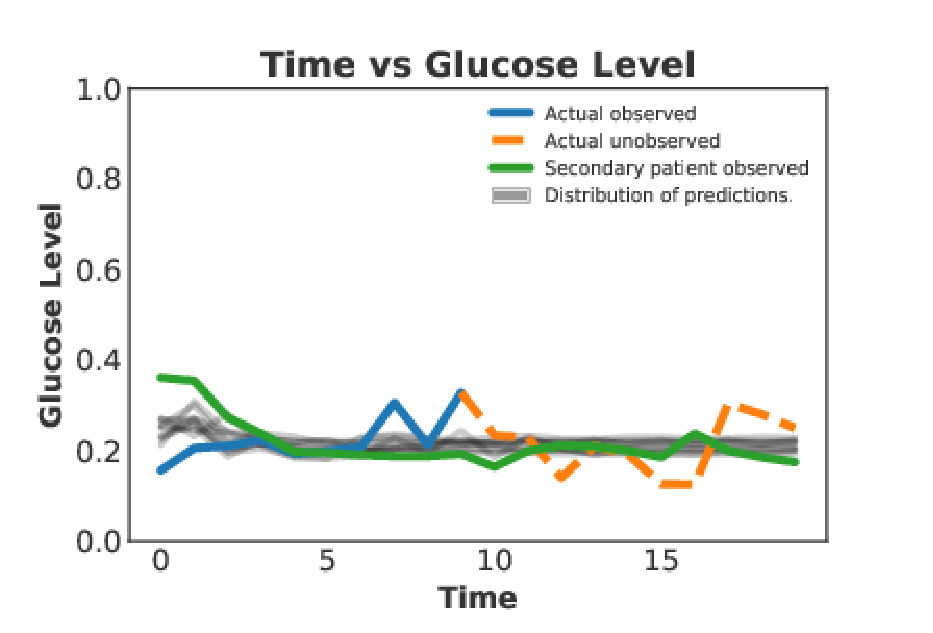
\includegraphics[width=0.7\linewidth, trim={1.cm, 0.1cm, 1.3cm, .5cm}, clip]{rnnsamples-py}
	%\fbox{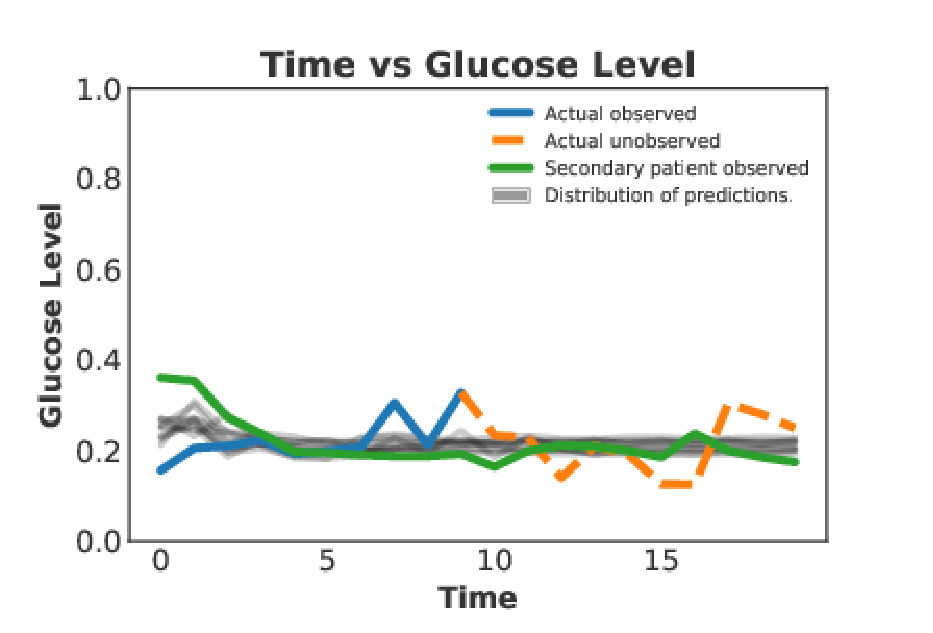
\includegraphics[width=0.30\linewidth, trim={1.cm, 0.1cm, 1.3cm, .5cm}, clip]{rnnsamples-py}}
	%\fbox{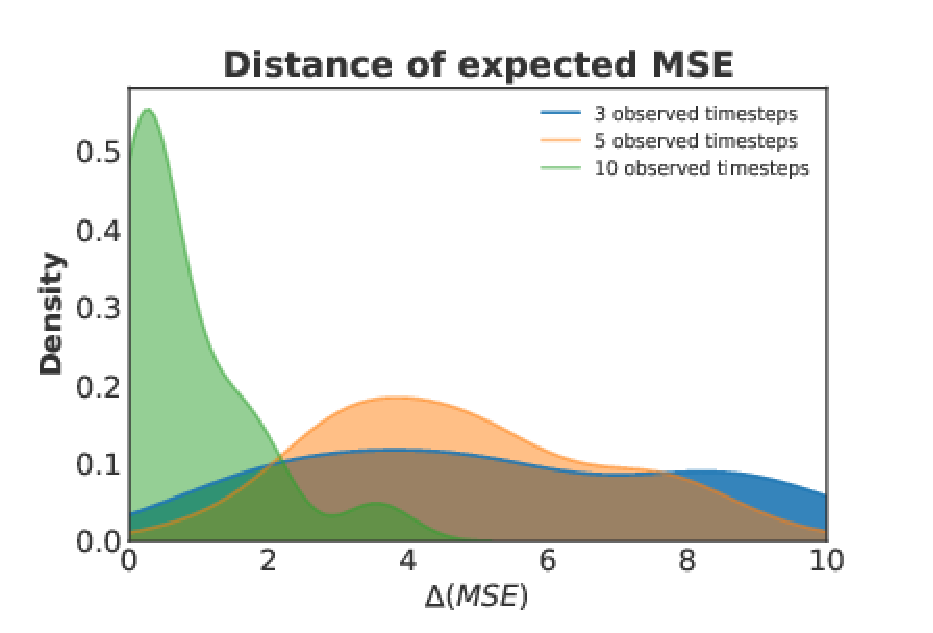
\includegraphics[width=0.30\linewidth, trim={1.cm, 0.0cm, 1.0cm, .5cm}, clip]{delta_mse}}
	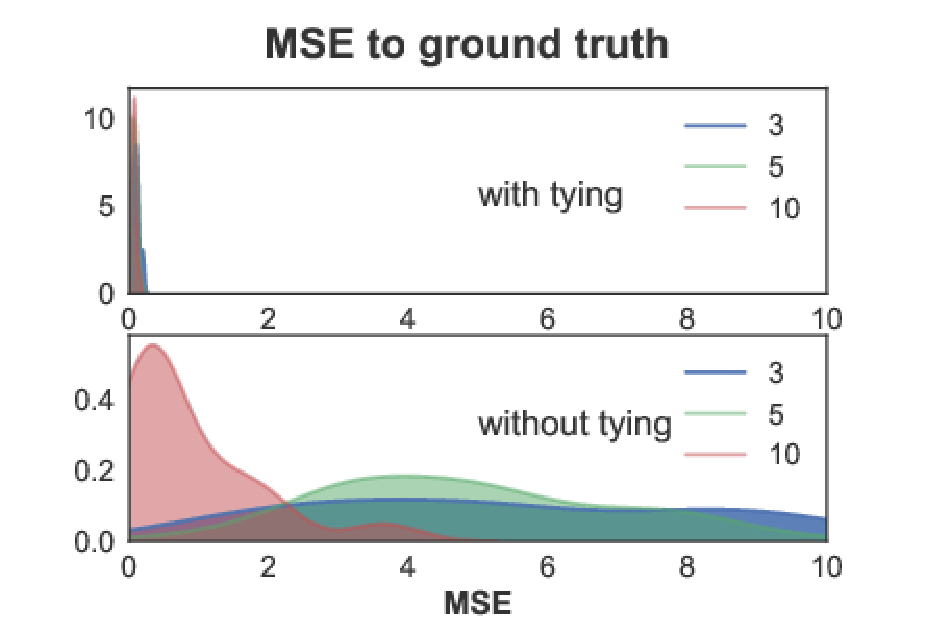
\includegraphics[width=0.7\linewidth, trim={0.7cm, 0.0cm, .7cm, .1cm}, clip]{mse}
		
		\caption{Top: Actual (dotted) and predicted trajectories that were learned using a partial trajectory. Center: Distribution of predicted trajectories learned only using the first ten data points and a tie with a secondary patient. Bottom, top: MSE when tie is present.  Bottom, bottom: without tie.  Tying expectations has dramatic influence on prediction error, while as more data is observed, the effect of tying decreases.}
		\label{fig:rnn-samples}
\end{figure}



% Take the same glucose measurements from 5 patients. Make a probabilistic RNN with
% independent parameters for each patient. Then add the constraint that the means are
% close. Then look at the prediction for one patient where we remove all but the
% first few time steps and show the forward predictions are better with the added knowledge
% that the means are close across patients.


% \paragraph{Transfer Learning}
% In transfer learning, we hope to use information from one learning problem to
% help with another learning problem. One way this has been accomplished in
% deep learning is to use
% the parameters of a model learned in one domain as the initialization for the
% parameters in a another domain. We could accomplish a similar thing via conditioning
% by having the weights of both models be close. But with conditioning, this is not
% the only choice, we can have the first layer activations be close in distribution
% in both the source and target transfer domain. Concretely, consider the following
% two layer stochastic neural network for each domain where the $i$th covariate
% label pair $(x_i, y_i)$ is
% \begin{align*}
% W \sim p(W)
% z_{2, i} &\sim p(z_{2, i} | x_i, W_2) \\
% z_{1, i} &\sim p(z_{1, i} | z_{2, i}, W_1) \\
% y_{i} &\sim p(y_i | z_{1, i})
% \end{align*}


% \section{Related Work}
% \begin{itemize}

% \item Existing Notion of Probablistic Programs
% Probabilistic programming languages and the inference algorithms which support them differ primarily in how probability distributions are represented.
% % In this contribution we define the sample space as an $n$-dimensional unit hypercube
% % $\Omega = [0, 1]^n$, and by $(\omega_1,...,\omega_n)$ denote an element of $\Omega$.
% % In addition, we define $\mu$ as the Lebesgue measure.
% % Random variables are transformations of $\Omega$, and act on some or all of its dimensions.
% % For example a random variable $\mathcal{U}_{a,b}: \Omega \to \mathbb{R}$, which is distributed uniformly between $a$ and $b$ could be defined simply as:
% % $$
% % \mathcal{U}_{a,b}(\omega) = a + \omega_1(b - a)
% % $$
% \item Make explicit how the measure theortic formulation connects to the sampling process
% \end{itemize}


\paragraph{Benchmarks}
To quantitatively compare predicate exchange with existing approaches we constructed an artificial problem that scales in difficulty.
Let $X_i \sim \mathcal{N}(0,1)$ in a $d$-dimensional model $\vect{X} = (X_1, \dots, X_d)$ conditioned on an $\epsilon$-thick ring:
\begin{equation}
\lk_\epsilon(\vect{x}) = 1 < |\vect{x}| < 1 + \epsilon
\end{equation}

Table \ref{results} compares the sample average of particle Gibbs (PG), sequential Monte Carlo (SMC), rejection sampling (RS) and predicate exchange (PE), varying both $\epsilon$ and $d$.
The theoretical expectation of all models is 0.
Among these methods, predicate exchange is unique in its support for inference with predicates, which makes direct comparison difficult.
For all inference procedures we use predicate relaxation to compute $d = \softv{\lk}_\epsilon(\vect{x})$, and sample from $\vect{X}$ conditioned on $\mathcal{N}(d, 1/(2\alpha)) = 1$, where $\alpha$ is the lowest temperature used in predicate exchange.
Predicate exchange  compares favourably in most scenarios.


\begin{figure}
\begin{center}
	\begin{tabular}{||c| c c c c||} 
	\hline
	 $d,\epsilon$& $1, {10^{-1}}$ & $1, {10^{-5}}$ & ${100}, {10^{-1}}$ & ${100}, {10^{-5}}$ \\ [0.5ex] 
	\hline\hline
	PE & 0.0054 & 0.4735  & -0.00037 & 0.00854\\ 
	\hline
	% HMC & 2.1 & 2.026  & 1.5 & 1.41\\ 
	% \hline\hline
	SMC & 0.06 & -0.226  & -0.018 & 0.09\\ 
	\hline
	PG & -0.029 & 0.239 & -0.03 & 0.03\\
	\hline
	RS & 0.003 & timedout & timedout & timedout \\
	\hline
 \end{tabular}
 \label{results}
 \caption{Comparison of expectations of samples from $d$ dimensional ring.  Theoretical value is 0 in all cases.}
 \end{center}
\end{figure}


  
\section{Related Work}

% Likelihood free inference
Demand for likelihood-free inference emerged in genetics ecology; Tavar{\'e} et al. \citep{tavare1997inferring} computed summary statistics of the output of a simulation, reject an accept-reject for posterior inference.
Weiss et al. \cite{weiss1998inference} expanded on this with a tolerance term, such that simulations yielding data sufficiently close to the targets were accepted.
Such posterior samples are therefore approximate.
Approximate Bayesian Computation (ABC) has come to refer to broad class of methods \cite{beaumont2002approximate,sisson2007sequential} in this general regime.
Marjoram et al. \cite{marjoram2003markov} simulated Markov Chains according to the prior, but introduced the accept/reject stage to yield approximate posterior samples.
A small tolerance leads to a high rejection rate, whereas a large tolerance results in an unacceptable approximation error.
Among several solutions are dynamically decreasing of tolerance \cite{toni2008approximate}, having a large tolerance but importance reweighting samples based on distance \cite{wegmann2009efficient}, adapting the tolerance based on the current distance \cite{del2012adaptive,lenormand2013adaptive}, as well as annealing the tolerance as a temperature parameter.

Predicate exchange targets simulation models and uses distance metrics, but targets exact inference without summary statistics.
In a recent approach with similar motivation, \cite{graham2017asymptotically} develop Hamiltonian Monte Carlo variant, which at each iteration uses a quasi-Newton method to solve exactly the constraint that the data is equal to the output of the generative model.  They perform HMC in an unconstrained space and project back to the constrained manifold.
This is costly -- although the cost is more than accounted for in a reduction of the number of steps -- and limited to differentiable models conditioned with equality. 

% \cite{Pseudo-Marginal Hamiltonian Monte Carlo}HMC methods cannot be implemented in scenarios where the likelihood function is intractable. However, we have shown here that if we have access to a non-negative unbiased likelihood estimator.
% parameterized by normal random variables then it is possible to derive an algorithm which mimicsthe HMC algorithm having access to the exact likelihood. The resulting pseudo-marginal HMCalgorithm replaces the original intractable gradient of the log-likelihood by the gradient of thelog-likelihood estimator while preserving the target distribution as invariant distributi

% PPLS
Probabilistic logics such as ProbLog \cite{richardson2006markov} and Markov logic networks \cite{de2007problog} extend first order logic with probabilistic constructs.
Predicate exchange conditions models on predicates belonging to a Boolean logic, but does not target logic languages in particular.
In fact, it is more suited to stochasticc simlator based models used in more recent probabilistic programming systems~\citep{milch20071, wood2014new,mansinghka2014venture,goodman2008church,carpenter2017stan}.  These systems automatically derive the likelihood function for a rich class of simulation based models, but are subject to the same restrictions that a tractaqble likelihood must exist.

% ?
% Our approach is related to smooth interpretation of programs \citep{chaudhuri2010smooth}

Several continuous logics have been developed to apply model-theoretic tools to metric structures which arise in analysis and geometry.
Continuous logics replace the Boolean structure ${T, F}$, quantifiers $\forall x$ and $\exists x$, and logical connectives with continuous functions,
but vary on the particular continuous structure uses
Predicate relaxation constructs predicates map to continuous structures, but departs from exiting work is primarily in motivation.
Our objective is not to provide a more general logic, but use continuity to make inference more tractable.
Semantically, our approach remains within measure theoretic foundations, which relies on hard predicates to condition.
Probabilistic Similarity Logic \cite{brocheler2012probabilistic,kimmig2012short} uses continuous logics 
Talk about Soft logic




\section{Discussion}
In this work we expanded the class of predicates that probabilistic models can be conditioned on in practice.

Problems of this form appear in all forms of program analysis.
This problem is called the path explosion problem, since the number of possible paths often increases combinatorially with program size and runtime length.
Automated program testing, which is concerned with finding program paths that yield to failure has developed various strategies \cite{cadar2008exe, sen2005cute}.
% Broadly, these trace the execution of the program and derive in symbol form the branch constraints.
% These constraints are solved to force the execution into branches of the program that incur error states.
% These tools have been scaled to very large problems, in complex real world code.
% Two methods that use heuristics toguide path exploration are [4] (which attempts to explore paths that hit less-often executed statements.
Unlike automated testing, probabilistic inference has the stricter requirement of adhering to the true posterior distribution.
However, in predicate exchange, we have a latitude on all nonunitary values.
This opens up the potential for extending program analysis methods to the probabilistic domain in future work.

% The objective of this contribution is to expand the class of predicates that probabilistic models can be effectively conditioned on

% Our methodology falls broadly within the domain of approximate bayesian computation, in the sense that we equip spaces with a distance metric.
% At a high level, this can be understood as extracting more information out of a predicate, which unmodified provides only 0 or 1, which is insufficiently informative for any inference procedure to exploit.
% By an large, inference in high-dimensional models has been restricted to fininte dimensional continous models.
% This remains the case for our method, methods discrete models remain a challenge

% Control flow remains a challenging problem, for fundamental reasons.


% There are several inference strategies other than replica exchange MCMC that could be constructed onto of a relaxed predicate.
% Maximum posterior inference is the most immediate option, which would entail maximizing equation \ref{}.

% Black-box inference methods have gained significant traction due to how general, flexible, a vs grey box



% \section{mathkey (delete me, later)}

\begin{enumerate}
\item $X$ - arbitrary random variable
\item \item $\cM$ - a model
\item $Y$ - Predicate to condition on
\item $\soft{Y}$ - Relaxation of $Y$ 
\item $f$ - posterior density
\item $p$ - prior density
\item $\lk$ - approximate likelihood (mistake there)
\item $\soft{\textrm{op}}$ - Relaxation of predicate $\textrm{op}$
\item $\cond$ - Operator in simulation model for conditioning
\item $\soft{y}$ - Soft Boolean element, i.e. in $[0, 1]$
\item $\pi$ - Simulation program
\item $\mathbb{D}$ dictionary
\item $k_\alpha$ - relxation kernel, parameterized by $\alpha$
\end{enumerate}


\bibliography{bib}
\bibliographystyle{icml2019}

\end{document}
